\documentclass[12pt,letterpaper]{article}
\usepackage{amsmath,amsthm,amsfonts,amssymb,amscd}
\usepackage{fullpage}
\usepackage{graphicx}
\usepackage{lastpage}
\usepackage{enumerate}
\usepackage{fancyhdr}
\usepackage{hyperref}
\usepackage{mathrsfs}
\usepackage{xcolor}
\usepackage[margin=3cm]{geometry}
\setlength{\parindent}{0.0in}
\setlength{\parskip}{0.05in}
\include{pgffor}

% Edit these as appropriate
\newcommand\course{STA571/CS590.01}
\newcommand\semester{Spring 2014}                   % <-- current semester
\newcommand\papertitle{Gaussian Processes}                          % <-- paper title
% \newcommand\authoryear{Heller and Ghahramani, ICML, 2005}
\newcommand\yourname{Matt Dickenson}                % <-- your name
\newcommand\login{mcd31}                            % <-- your NetID
\newcommand\hwdate{Due: 21 March, 2014}           % <-- HW due date

% \newcommand\forparams[1,2,3]{
%   \begin{figure}
%   \begin{center}
%   \includegraphics{}
% }

\pagestyle{fancyplain}
\headheight 60pt
\chead{Gaussian Process Simulations\\ ~\\}
\lhead{\small \yourname\ \texttt{\login}\\\course}
\rhead{\small \hwdate}
\headsep 10pt

\begin{document}

% \noindent \emph{Homework Notes:} 

\section{Code}
The following code was used to generate (function) samples from Guassian processes using several covariance functions. The simulations are shown below. 

\lstinputlisting[caption=GP code, language=R, lastline=123]{3-21-homework-mcd.R}

\pagebreak
\section{Squared Exponential Covariance}

The simulations in this section use the squared exponential covariance function:
\begin{eqnarray*}
k(x, x^{\prime}) &=& \exp \{ - \frac{(x - x^{\prime})^2} {2 \ell^2 } \}
\end{eqnarray*} 

The parameters of interest here are the number of functions generated, $n$, the mean of the multivariate normal used for the simulations, $\mu$, and the length scale $\ell$. Each simulation plot shows the parameters used. 

\begin{figure}
\begin{center}
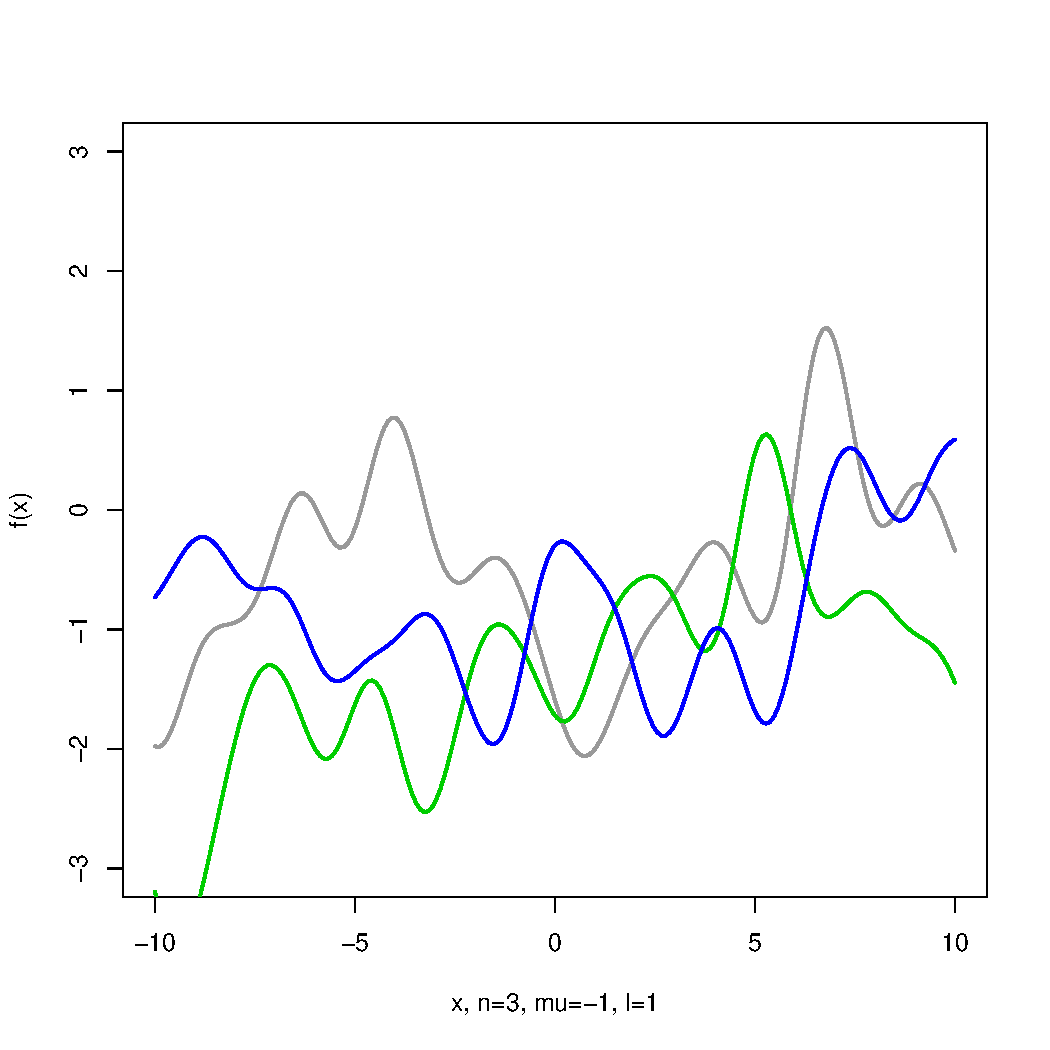
\includegraphics[scale=0.2]{hw321/n3-m-1-l1.pdf}
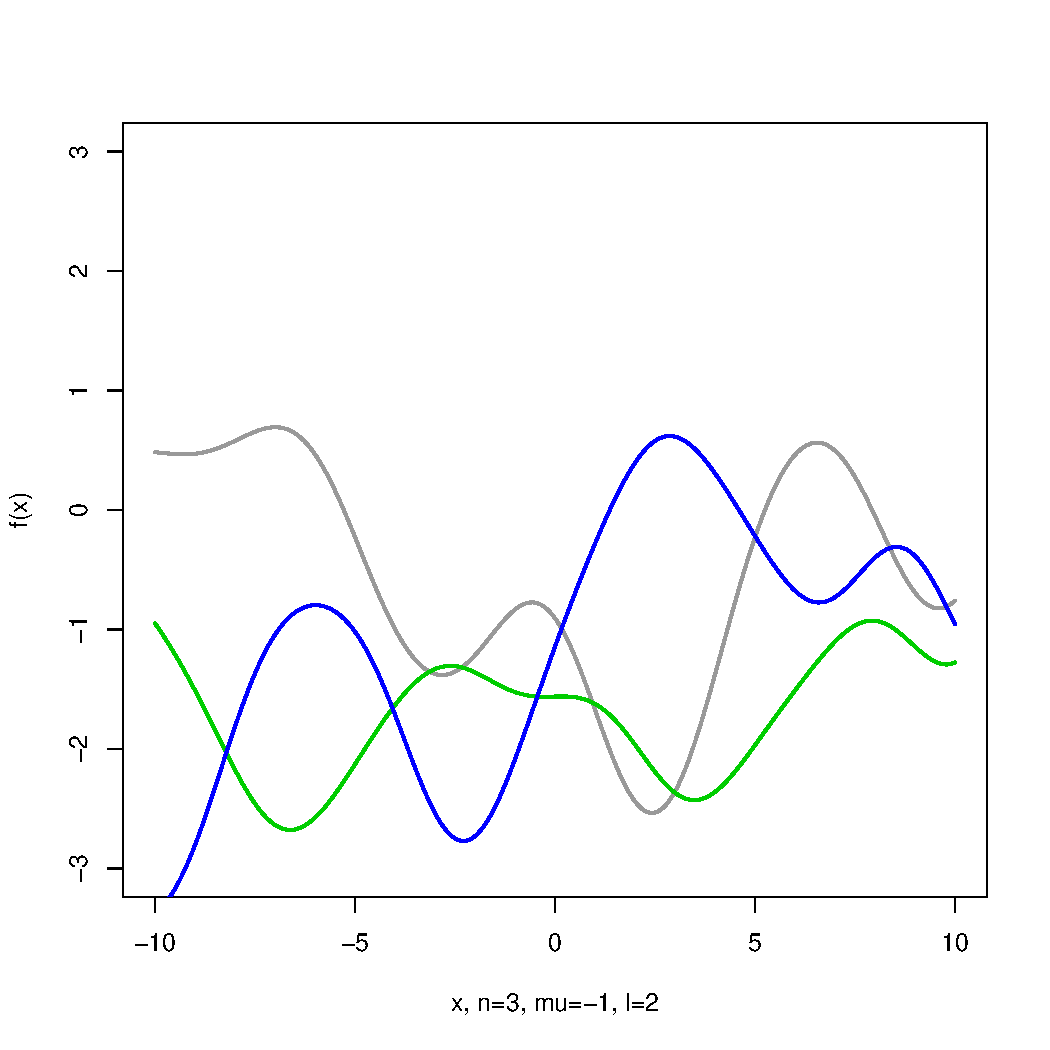
\includegraphics[scale=0.2]{hw321/n3-m-1-l2.pdf}
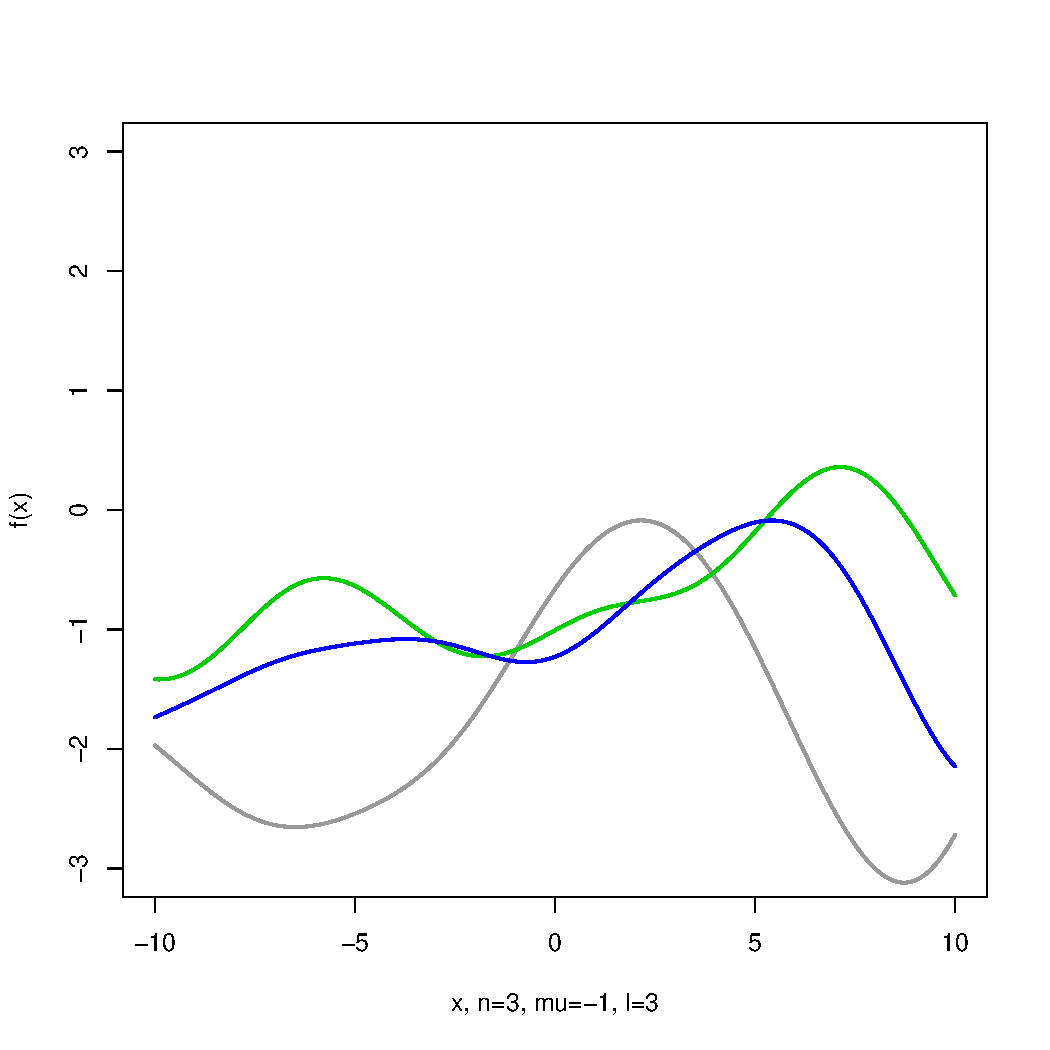
\includegraphics[scale=0.2]{hw321/n3-m-1-l3.pdf}
\end{center}
\end{figure}
\begin{figure}
\begin{center}
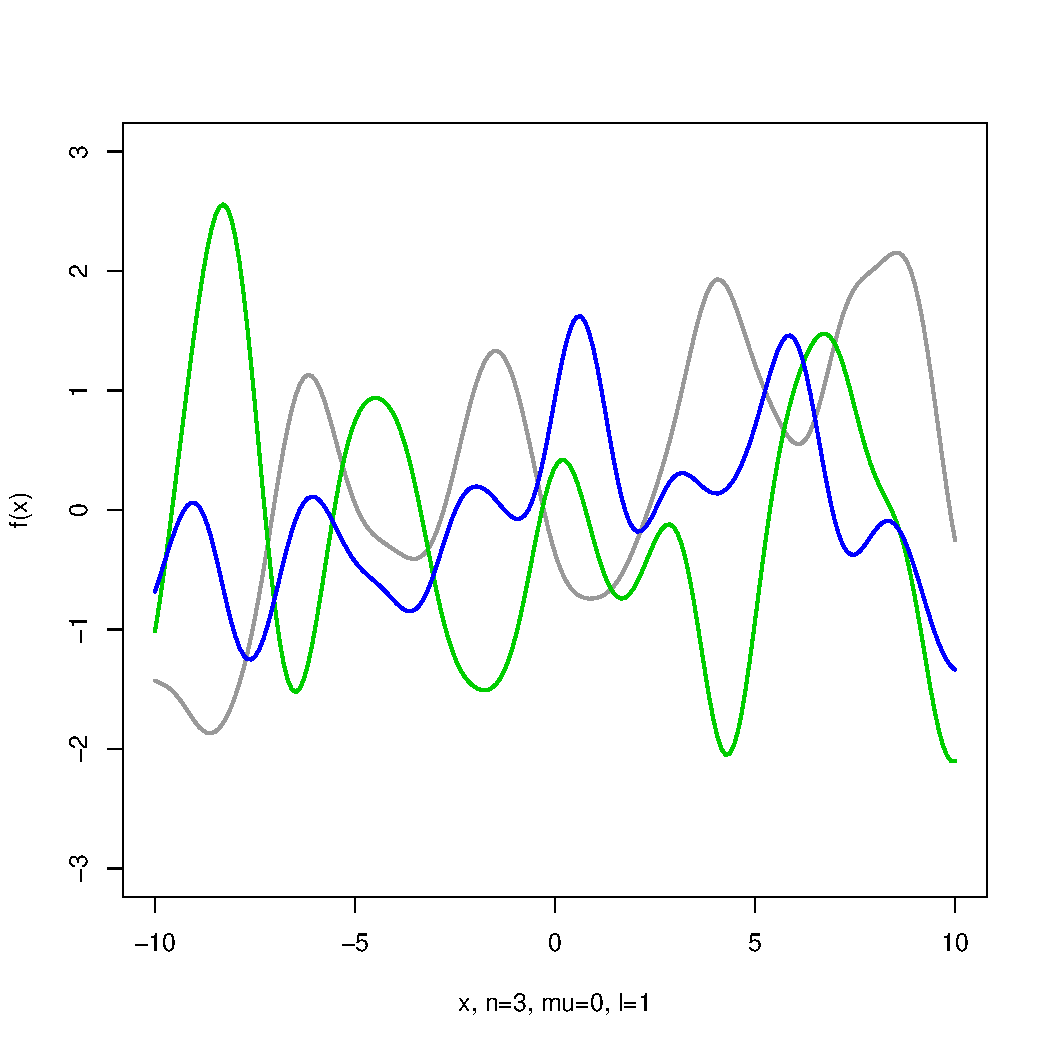
\includegraphics[scale=0.2]{hw321/n3-m0-l1.pdf}
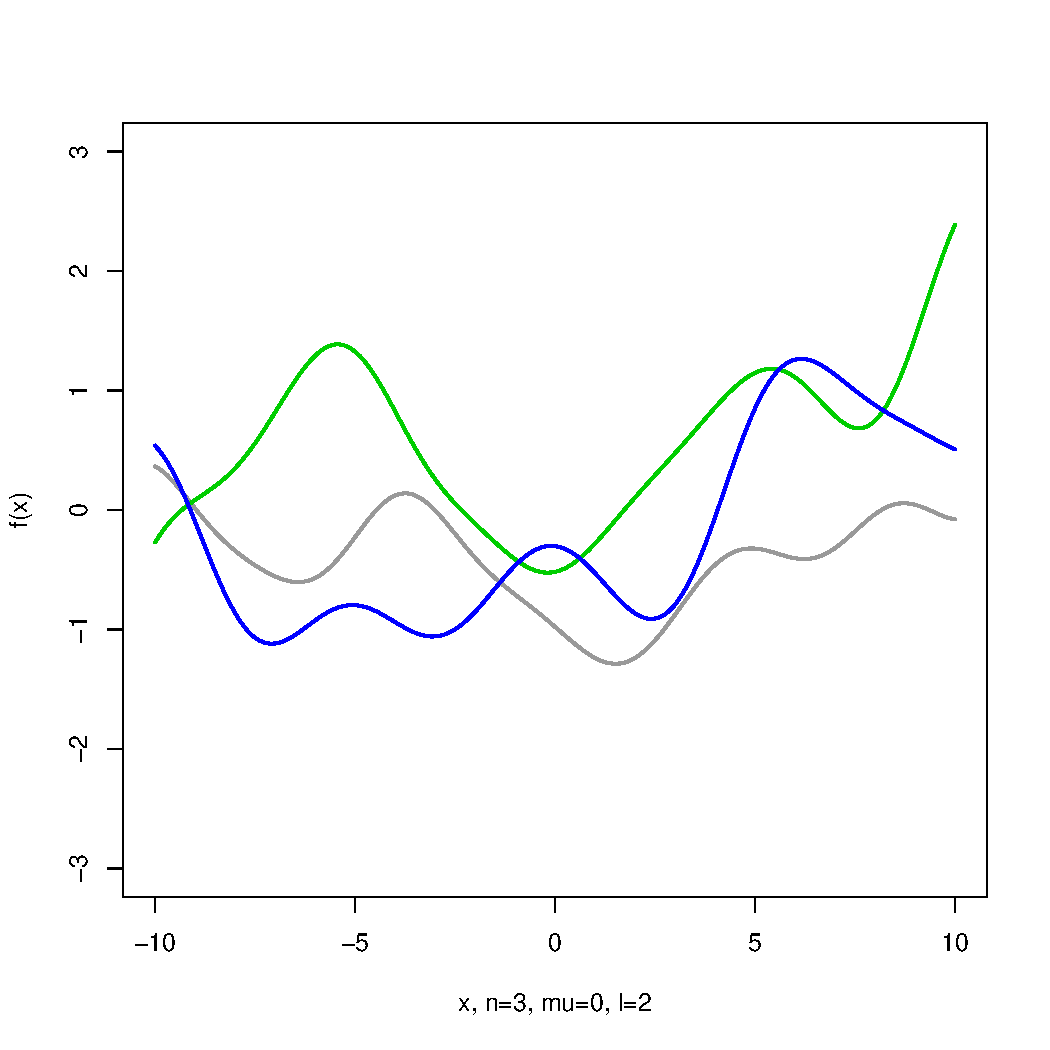
\includegraphics[scale=0.2]{hw321/n3-m0-l2.pdf}
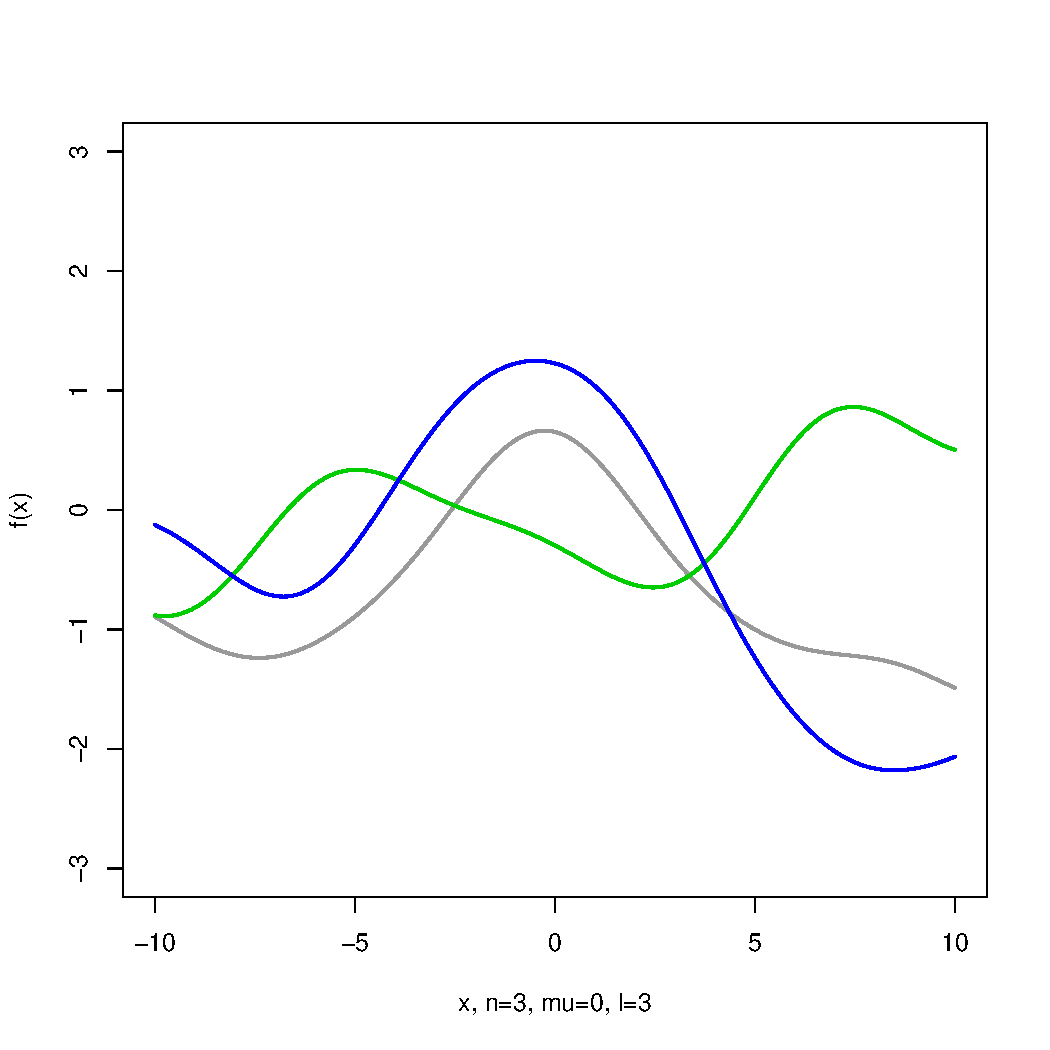
\includegraphics[scale=0.2]{hw321/n3-m0-l3.pdf}
\end{center}
\end{figure}
\begin{figure}
\begin{center}
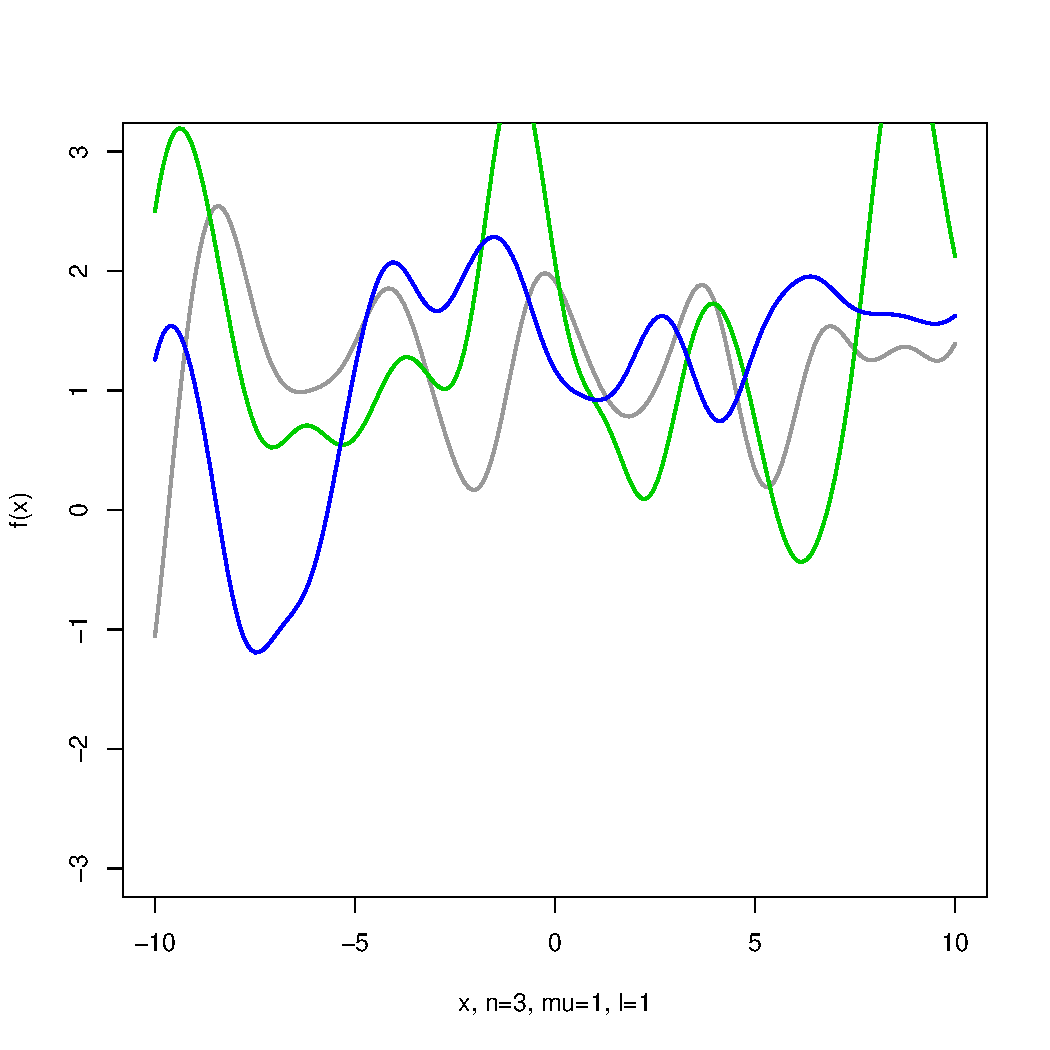
\includegraphics[scale=0.2]{hw321/n3-m1-l1.pdf}
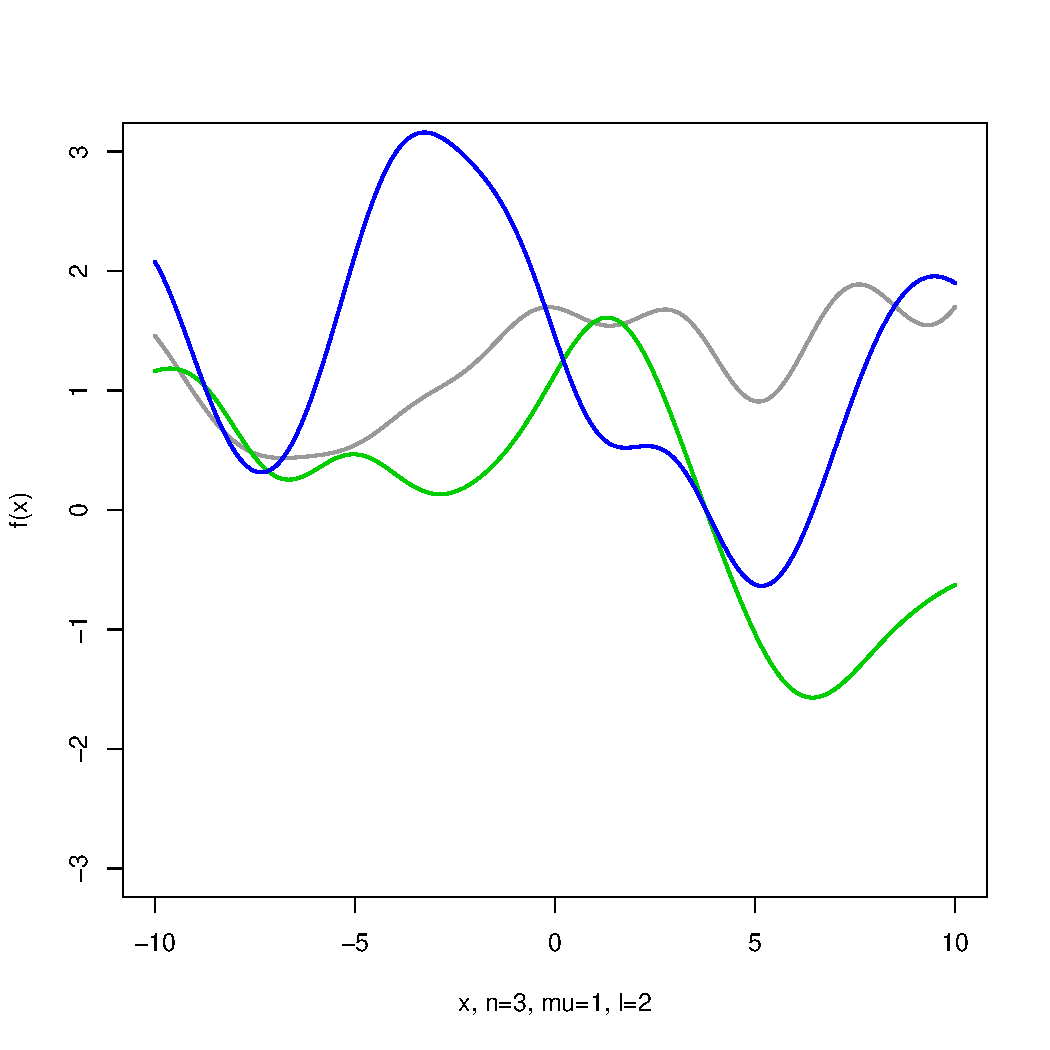
\includegraphics[scale=0.2]{hw321/n3-m1-l2.pdf}
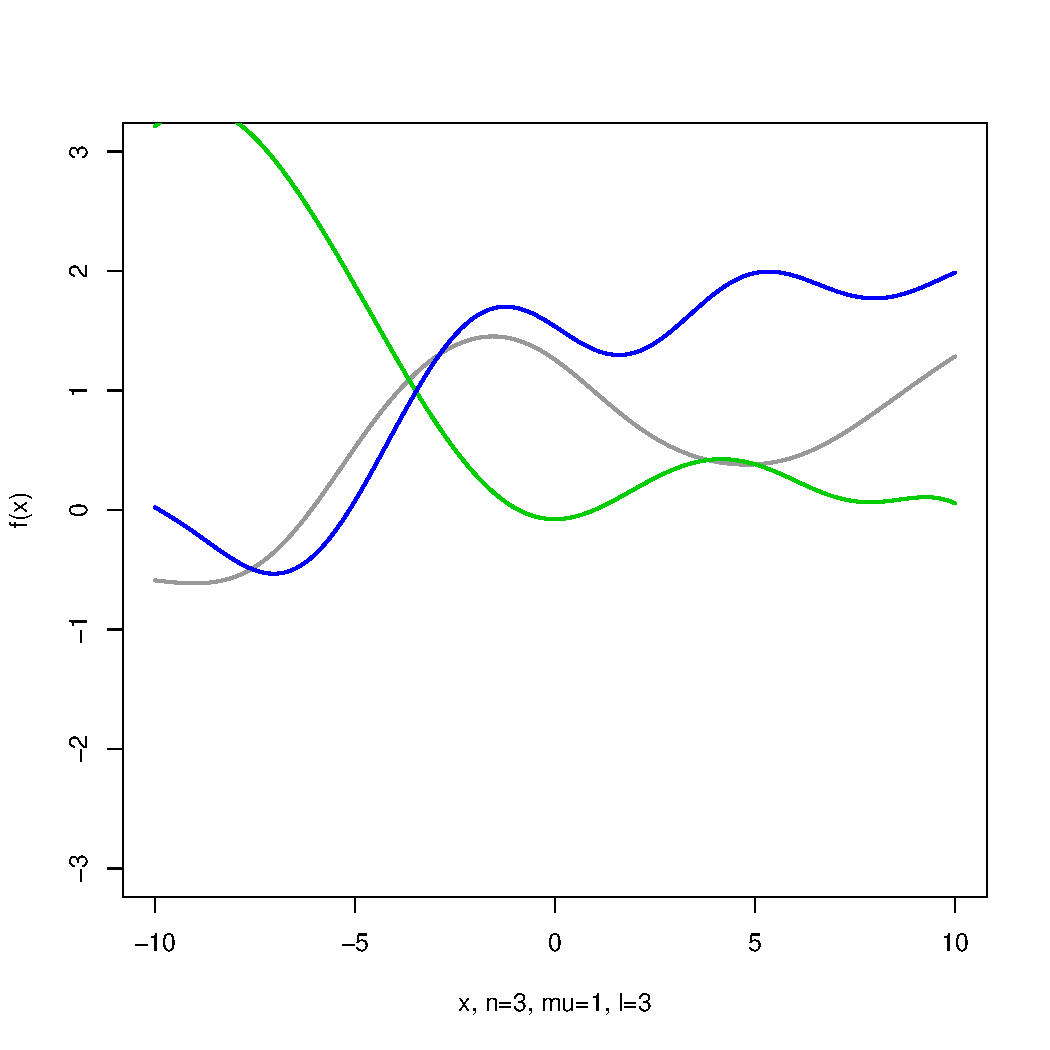
\includegraphics[scale=0.2]{hw321/n3-m1-l3.pdf}
\end{center}
\end{figure}
\begin{figure}
\begin{center}
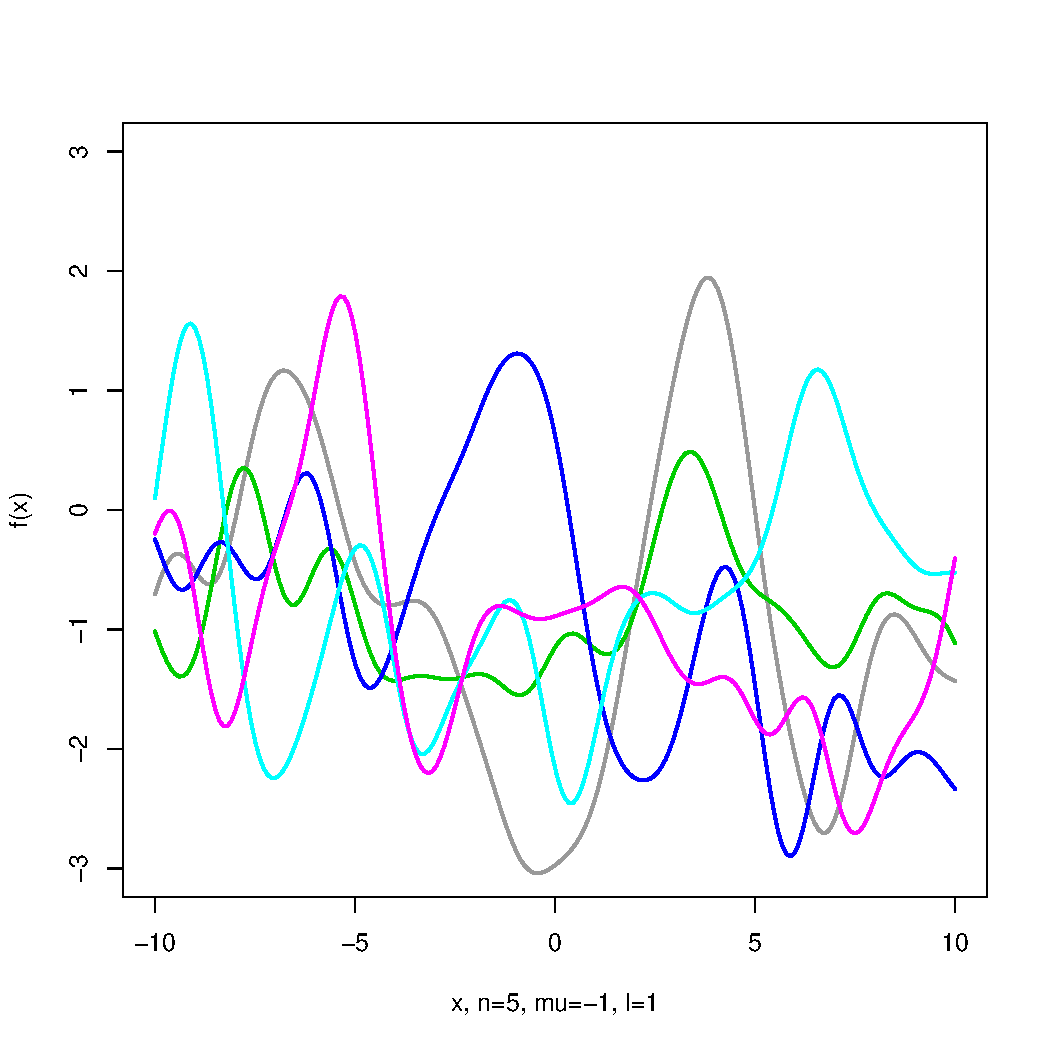
\includegraphics[scale=0.2]{hw321/n5-m-1-l1.pdf}
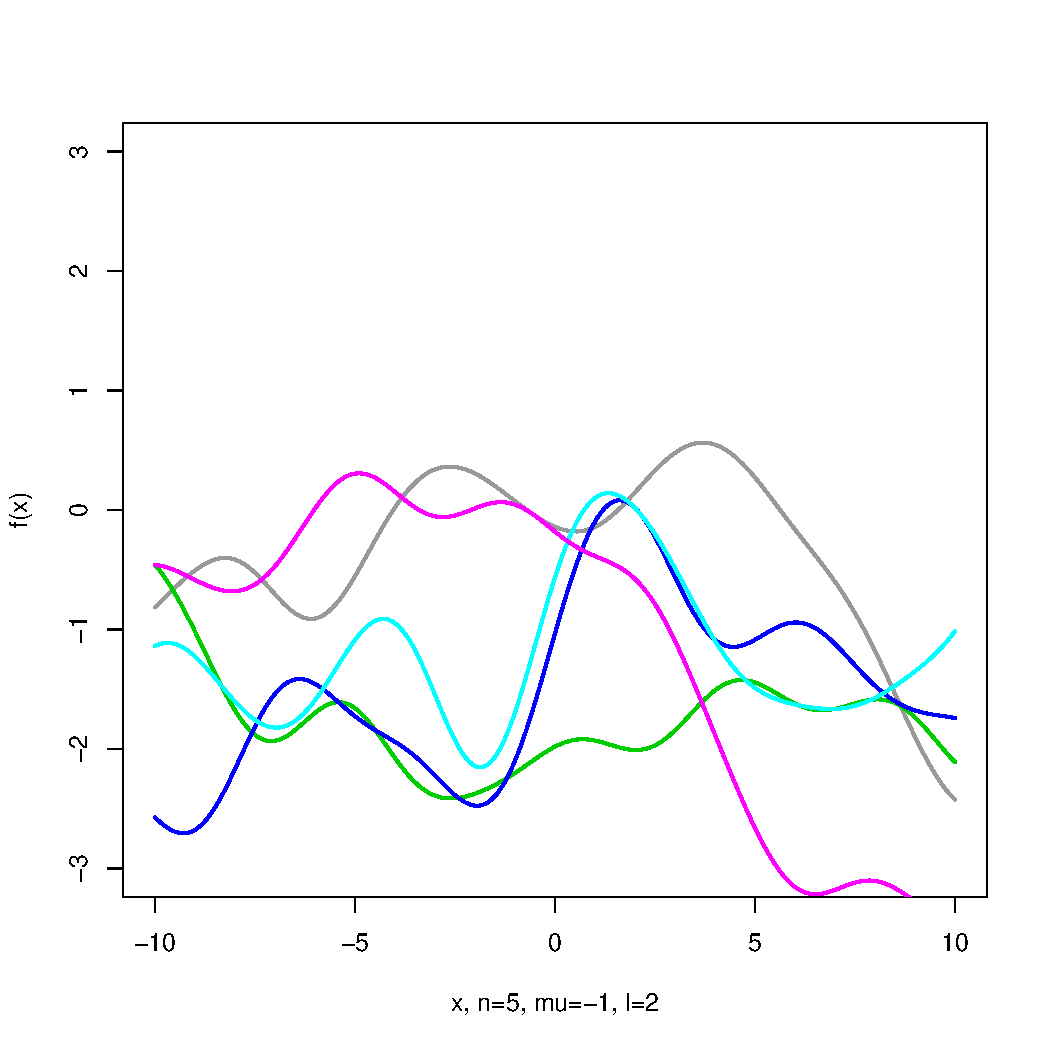
\includegraphics[scale=0.2]{hw321/n5-m-1-l2.pdf}
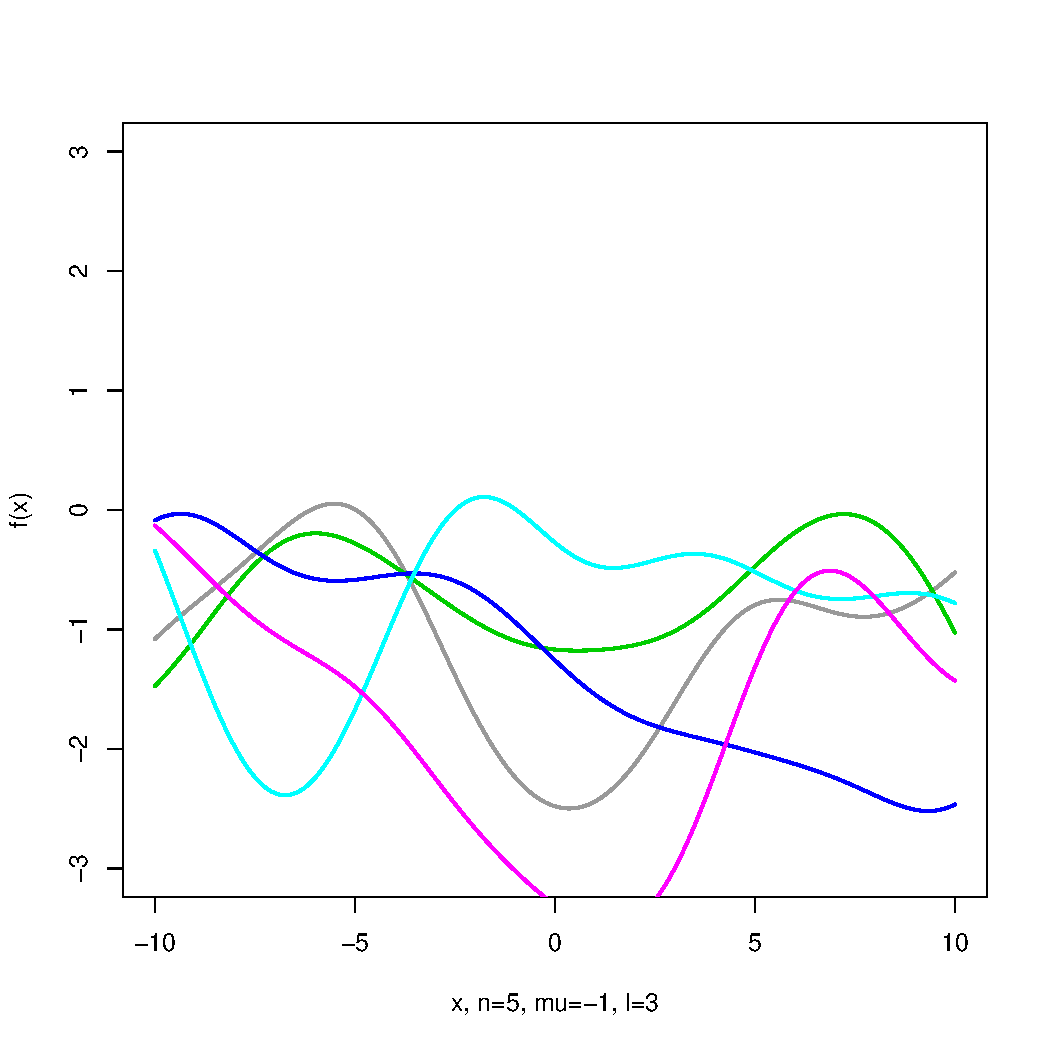
\includegraphics[scale=0.2]{hw321/n5-m-1-l3.pdf}
\end{center}
\end{figure}
\begin{figure}
\begin{center}
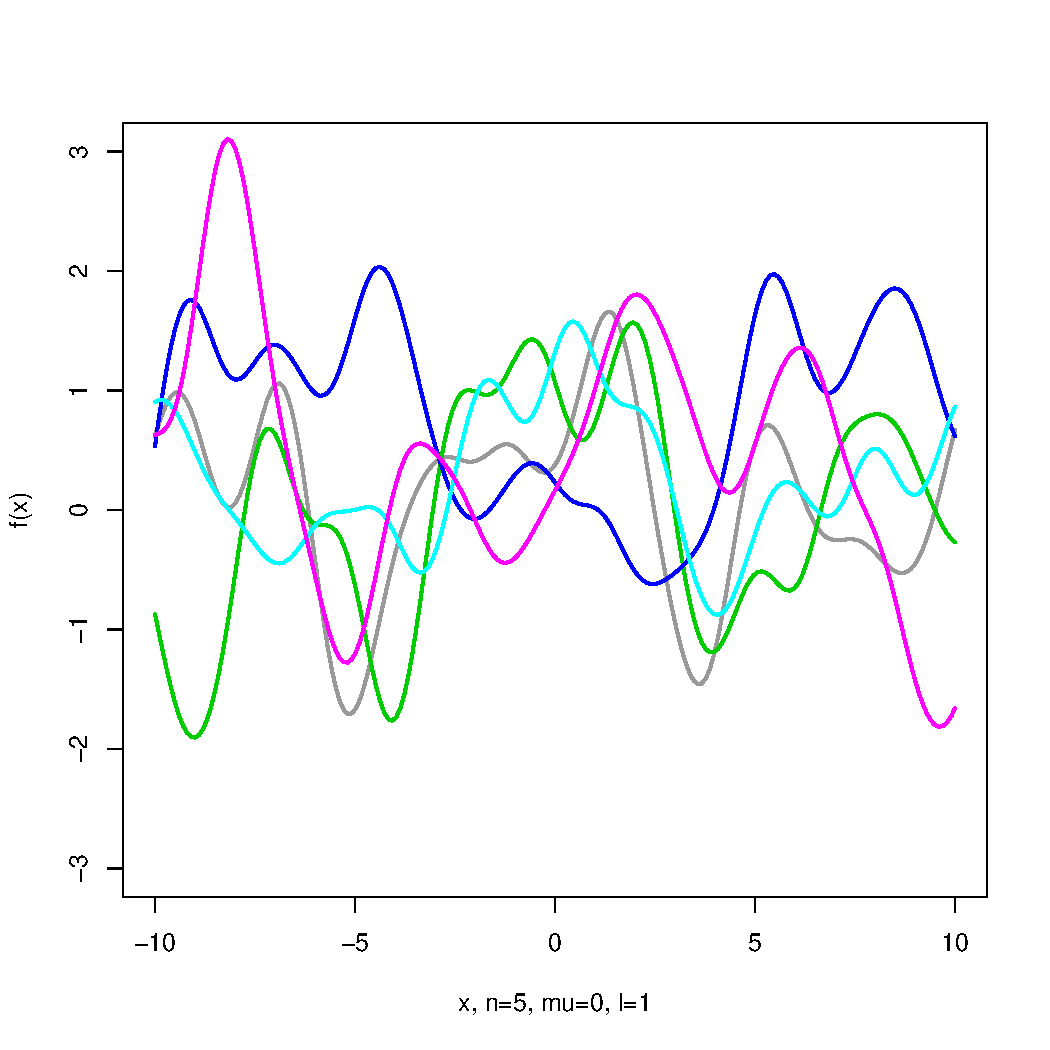
\includegraphics[scale=0.2]{hw321/n5-m0-l1.pdf}
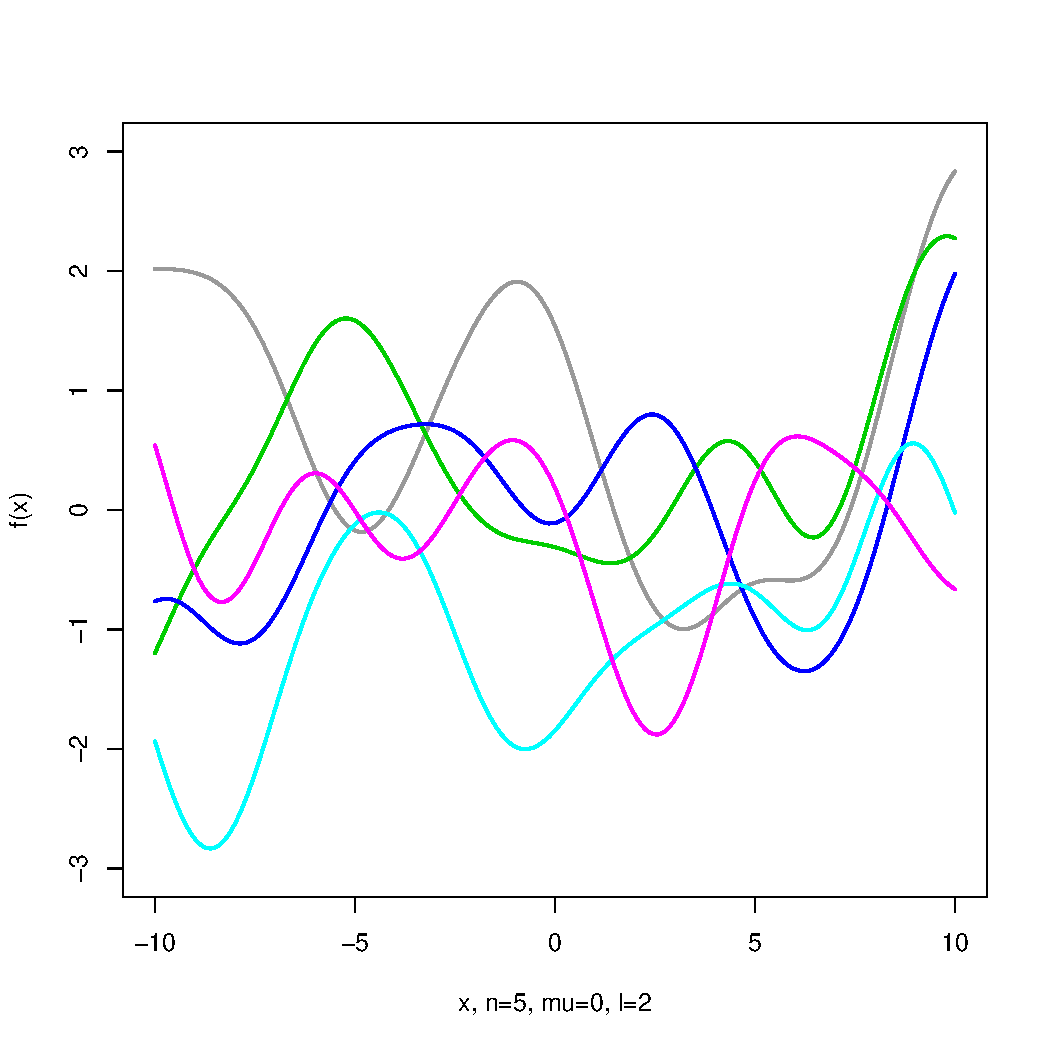
\includegraphics[scale=0.2]{hw321/n5-m0-l2.pdf}
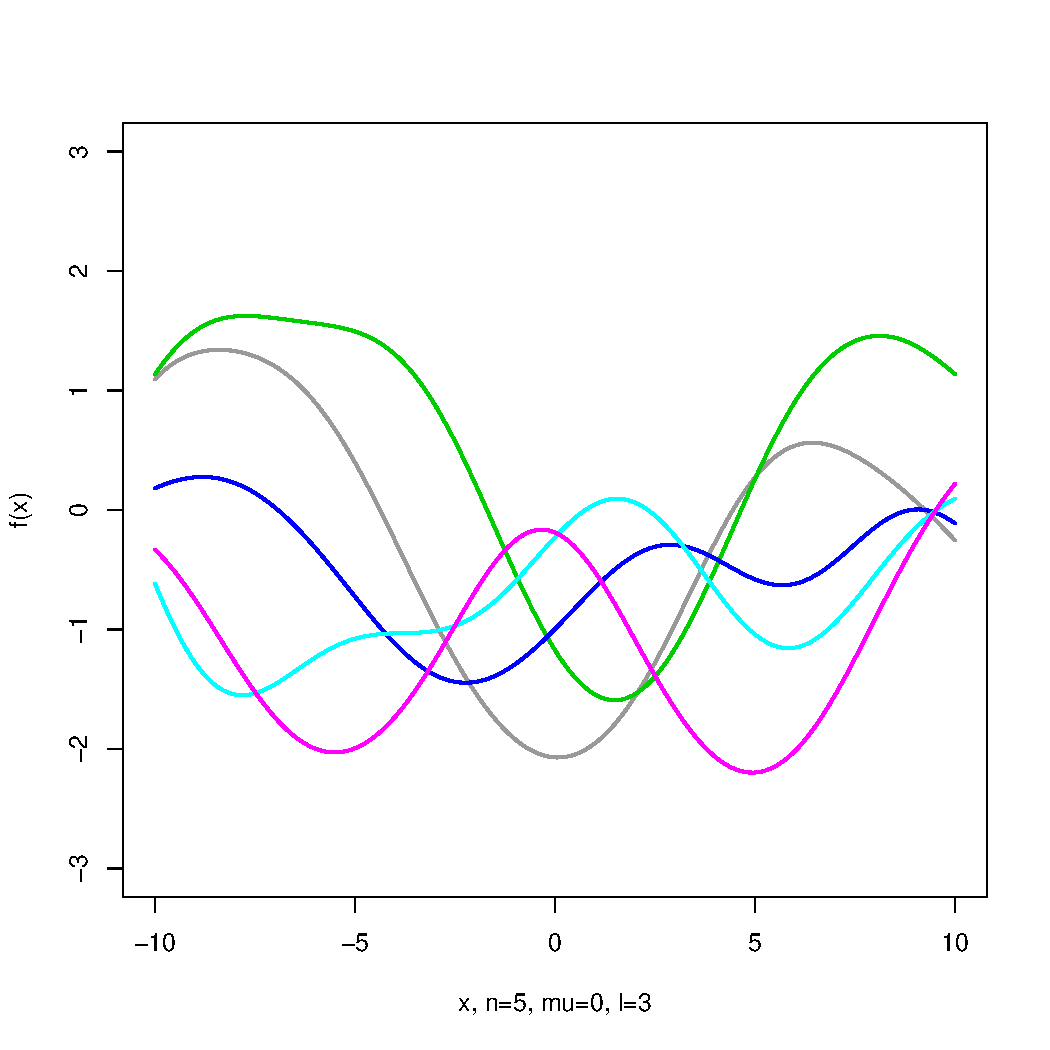
\includegraphics[scale=0.2]{hw321/n5-m0-l3.pdf}
\end{center}
\end{figure}
\begin{figure}
\begin{center}
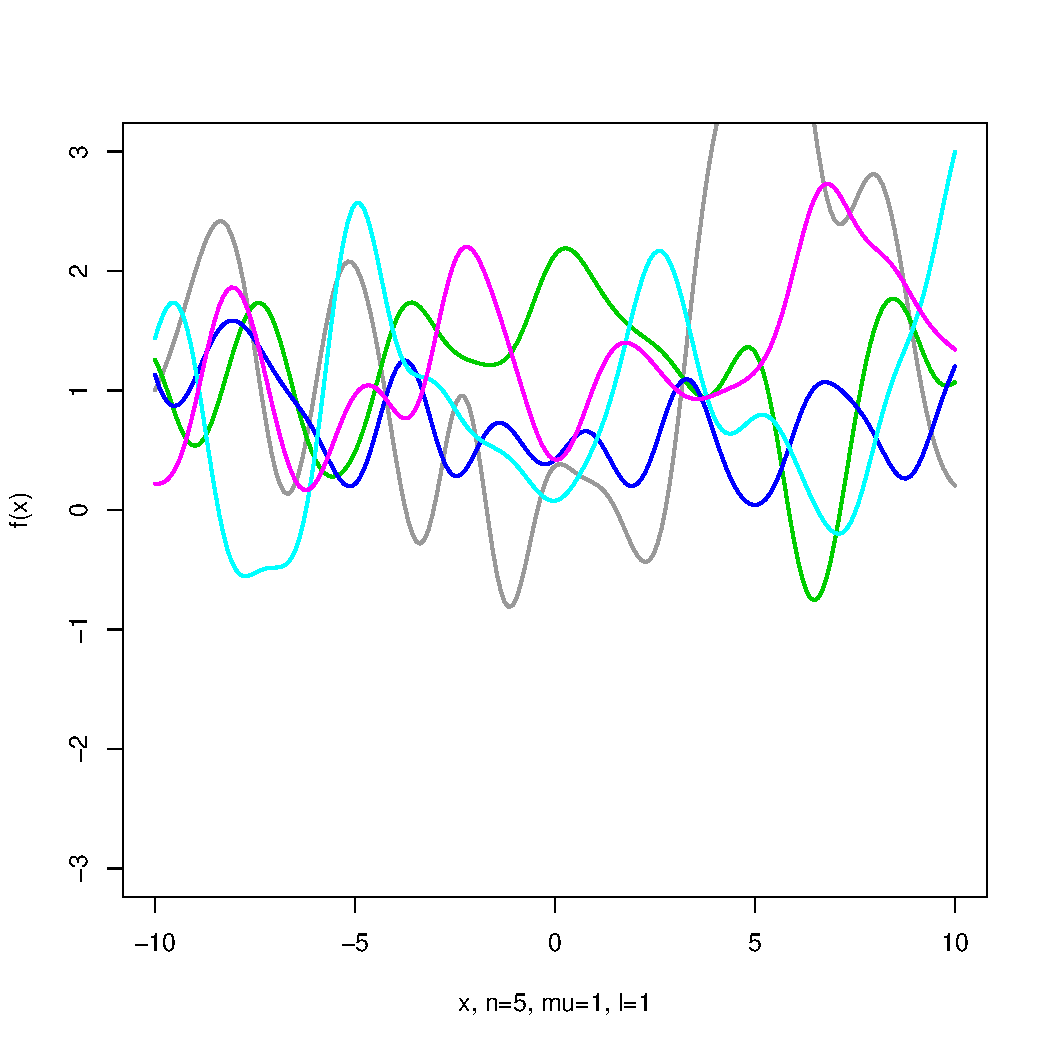
\includegraphics[scale=0.2]{hw321/n5-m1-l1.pdf}
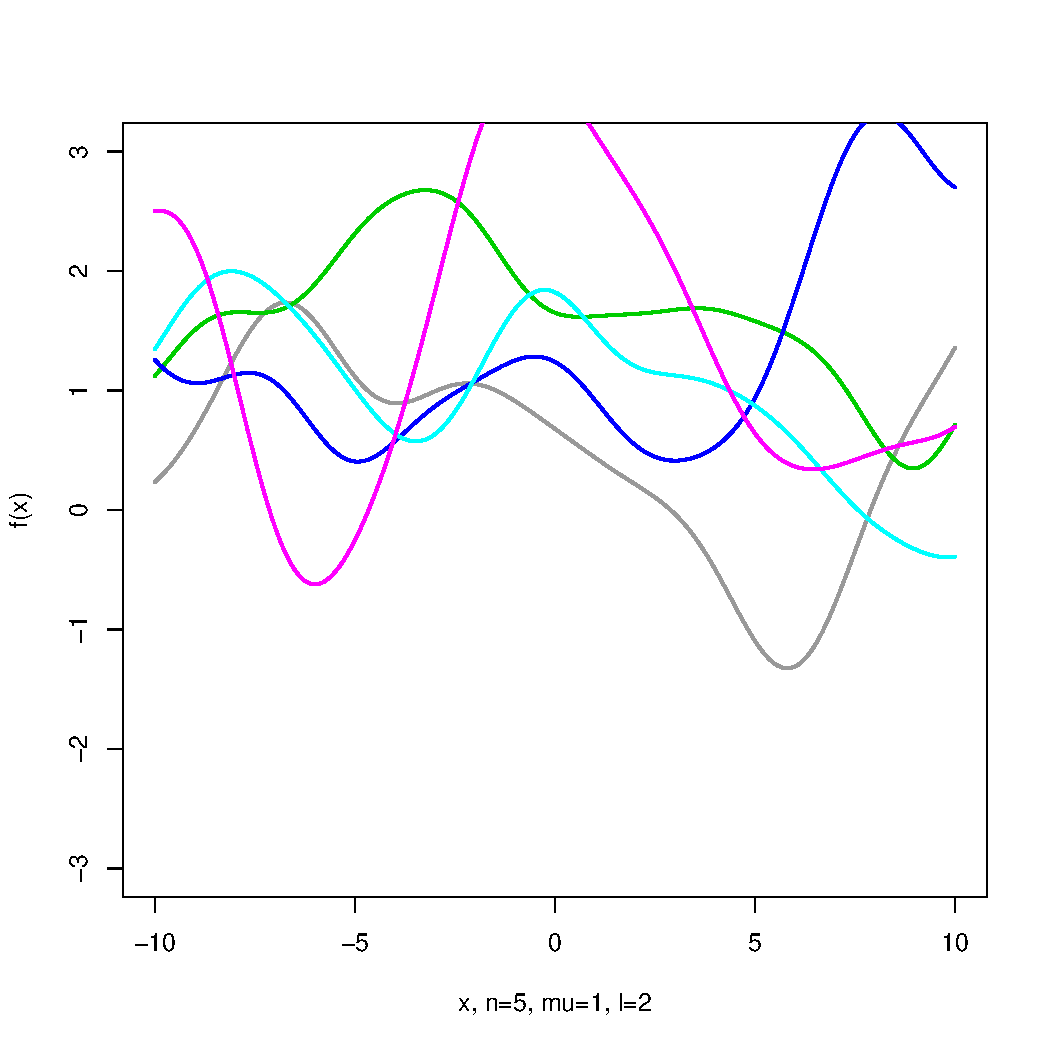
\includegraphics[scale=0.2]{hw321/n5-m1-l2.pdf}
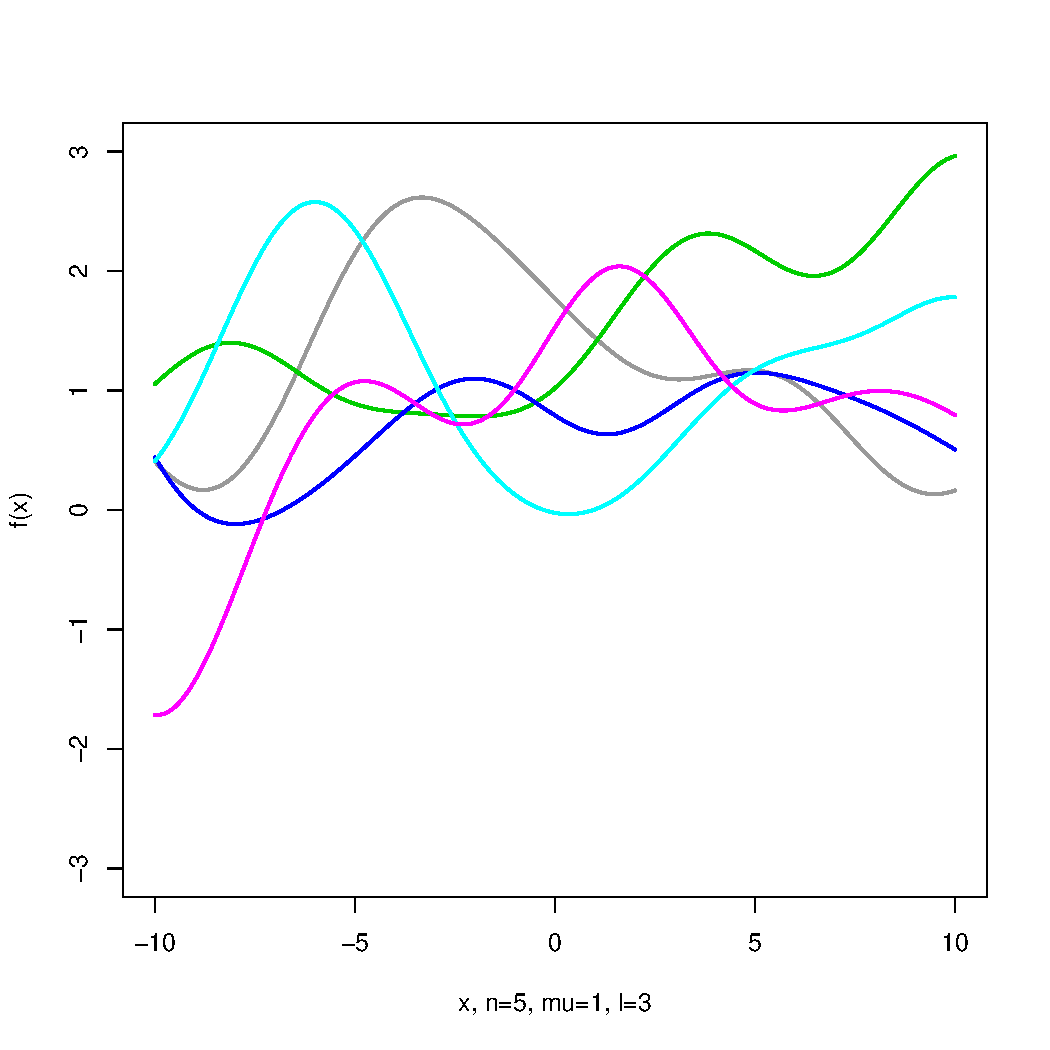
\includegraphics[scale=0.2]{hw321/n5-m1-l3.pdf}
\end{center}
\end{figure}
\begin{figure}
\begin{center}
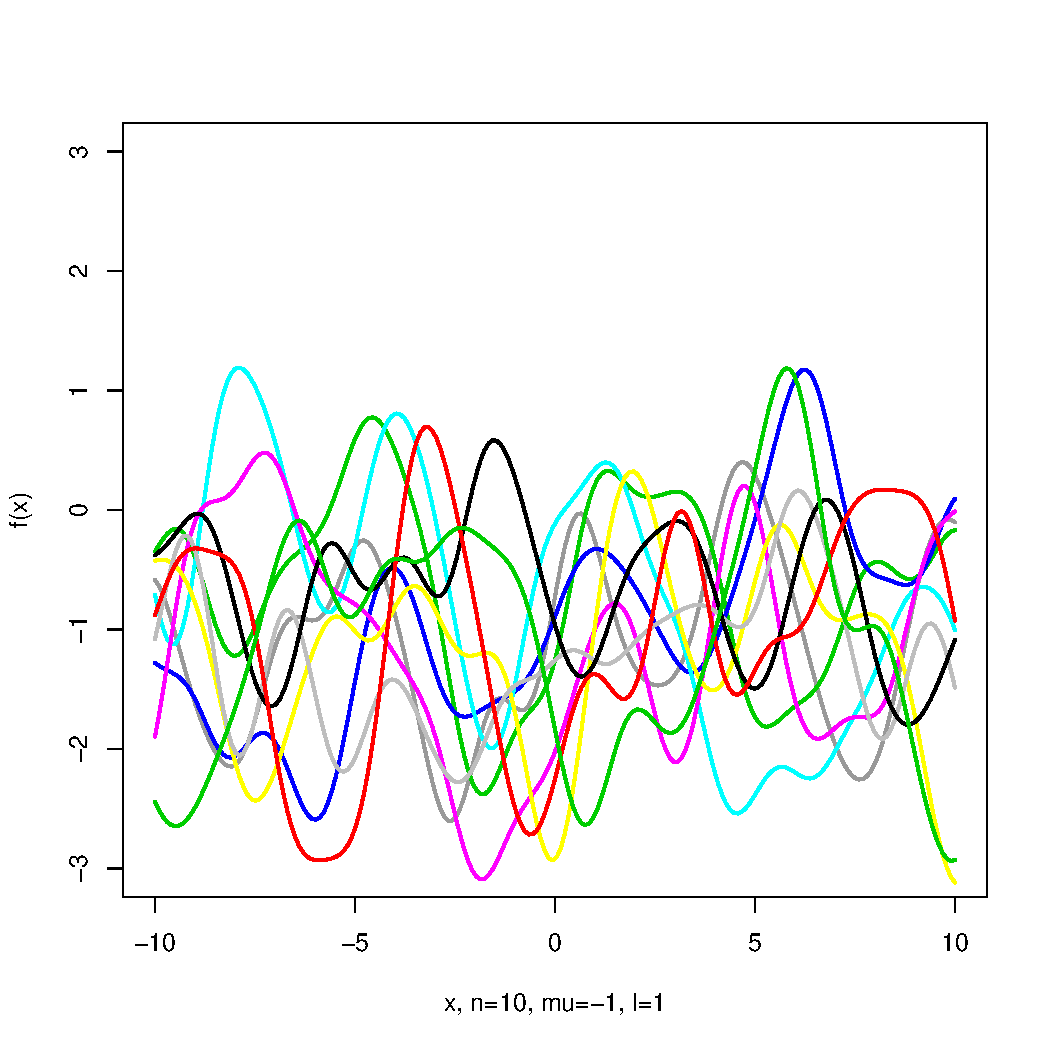
\includegraphics[scale=0.2]{hw321/n10-m-1-l1.pdf}
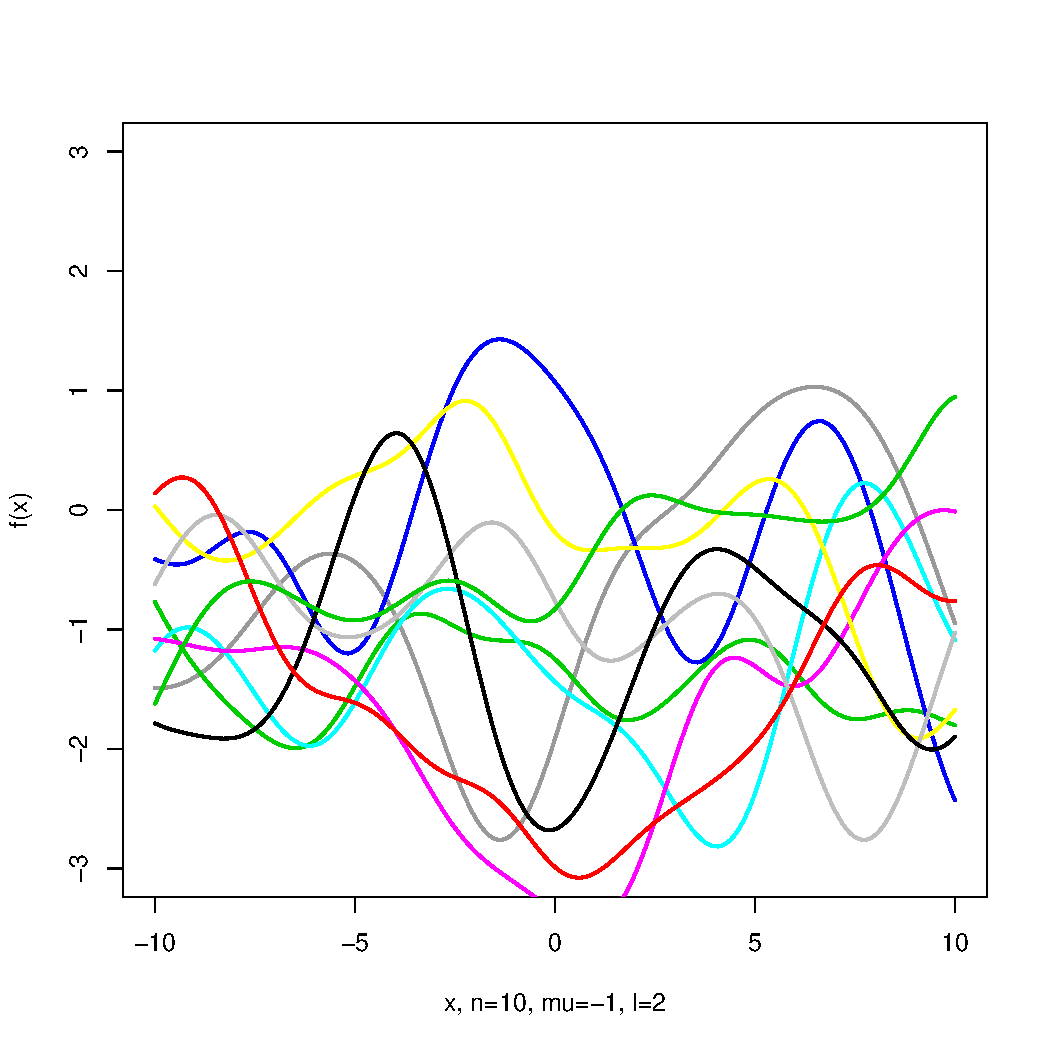
\includegraphics[scale=0.2]{hw321/n10-m-1-l2.pdf}
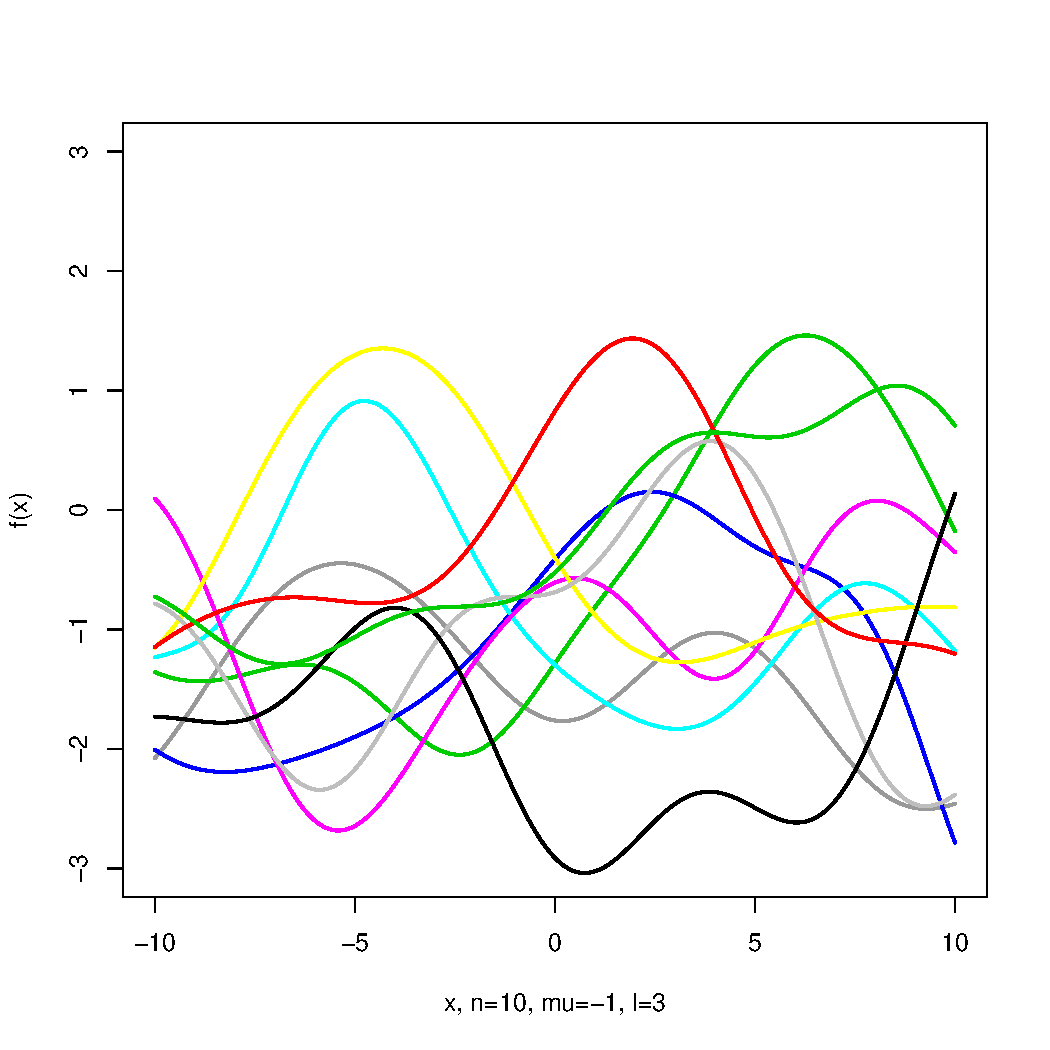
\includegraphics[scale=0.2]{hw321/n10-m-1-l3.pdf}
\end{center}
\end{figure}
\begin{figure}
\begin{center}
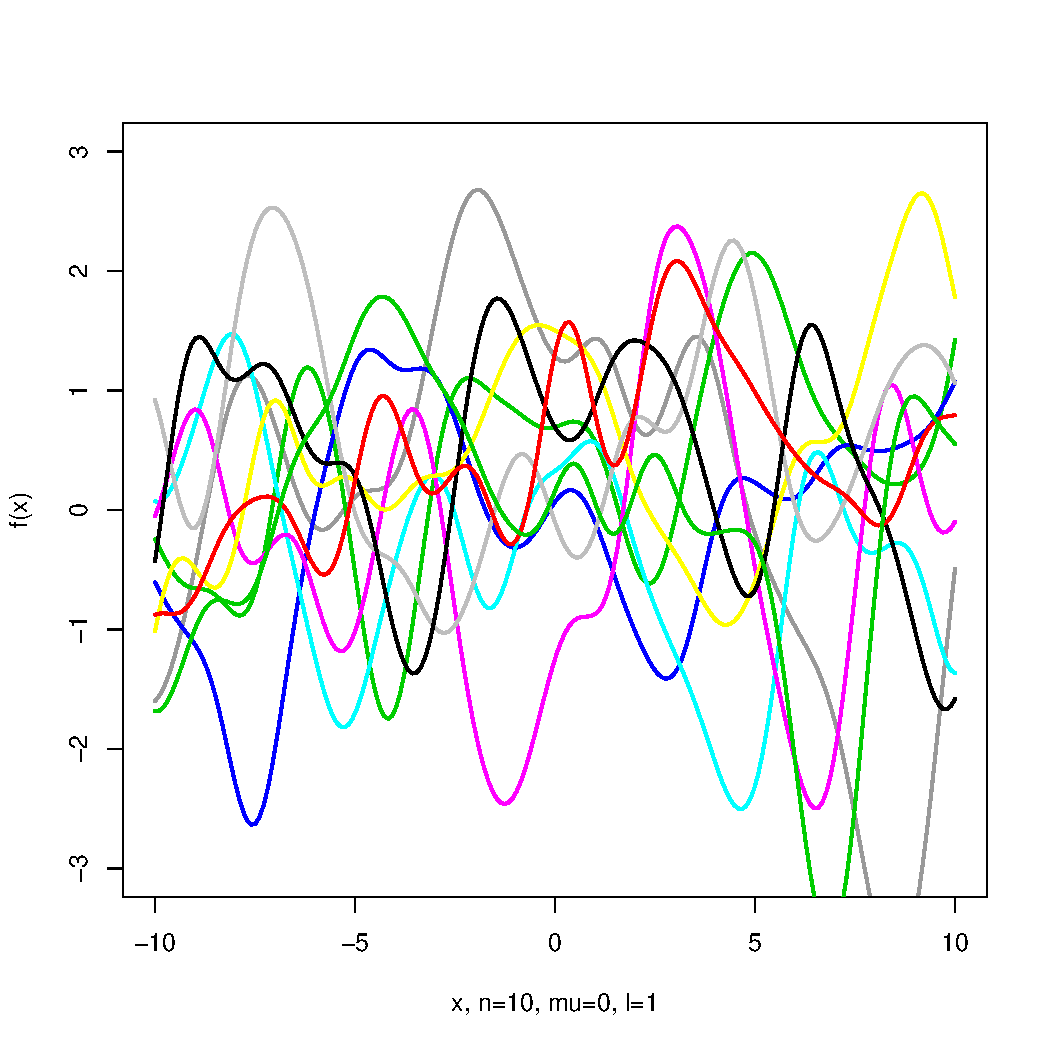
\includegraphics[scale=0.2]{hw321/n10-m0-l1.pdf}
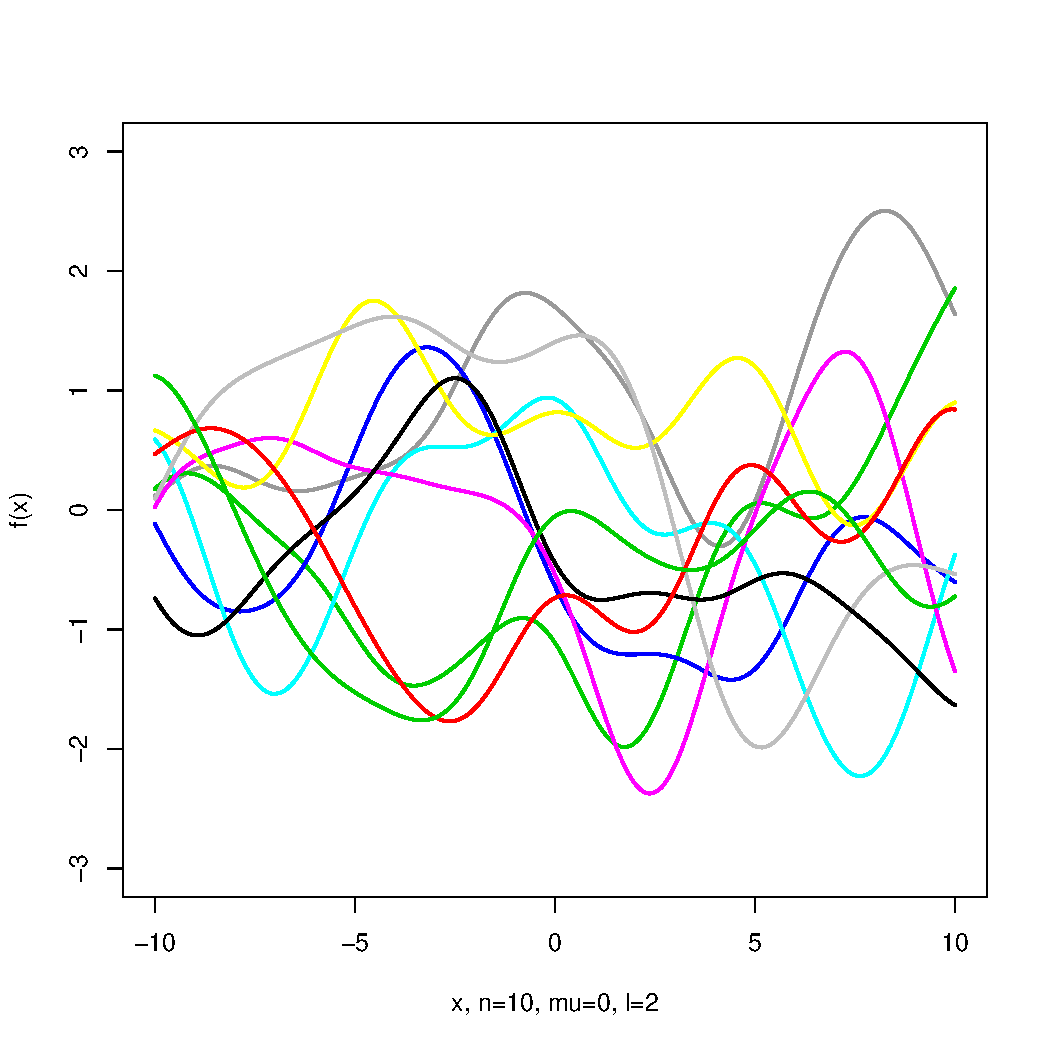
\includegraphics[scale=0.2]{hw321/n10-m0-l2.pdf}
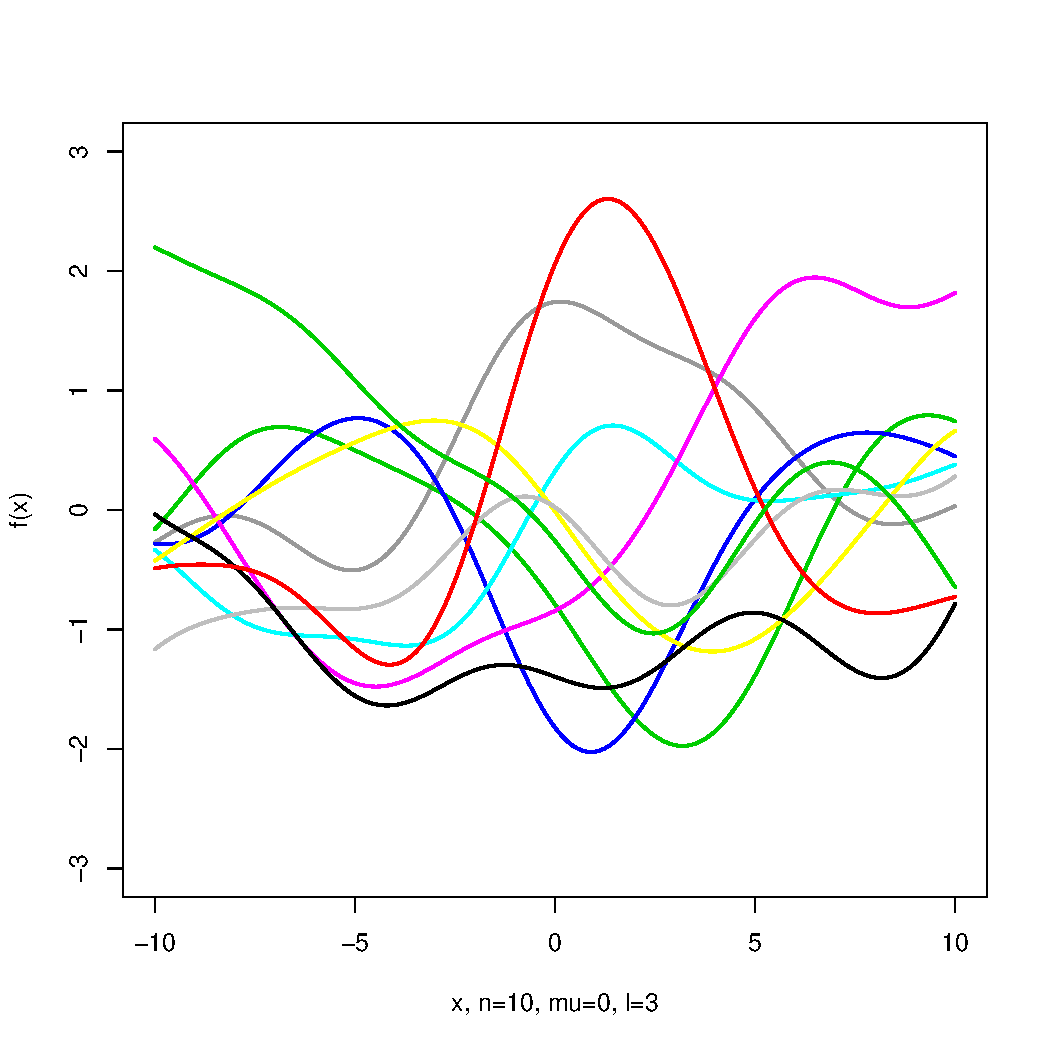
\includegraphics[scale=0.2]{hw321/n10-m0-l3.pdf}
\end{center}
\end{figure}
\begin{figure}
\begin{center}
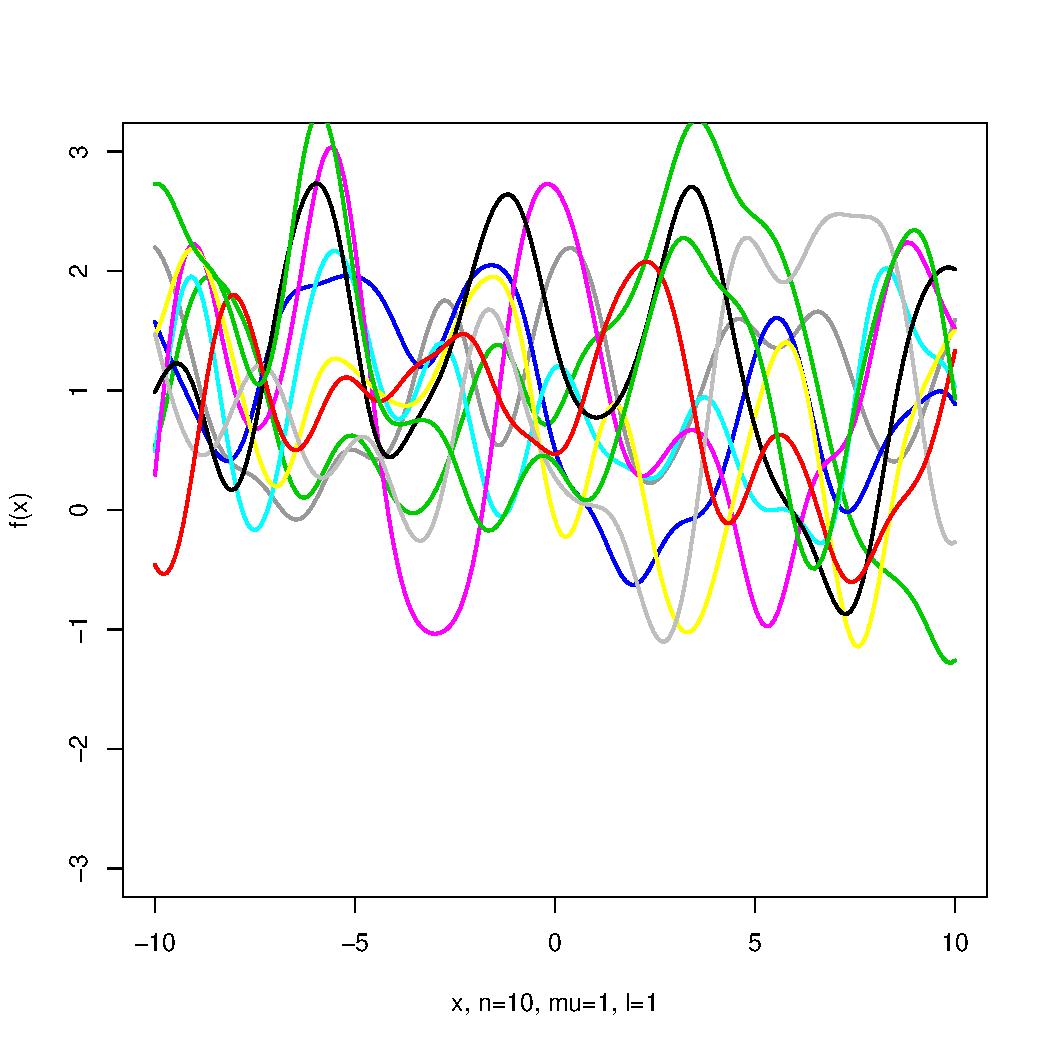
\includegraphics[scale=0.2]{hw321/n10-m1-l1.pdf}
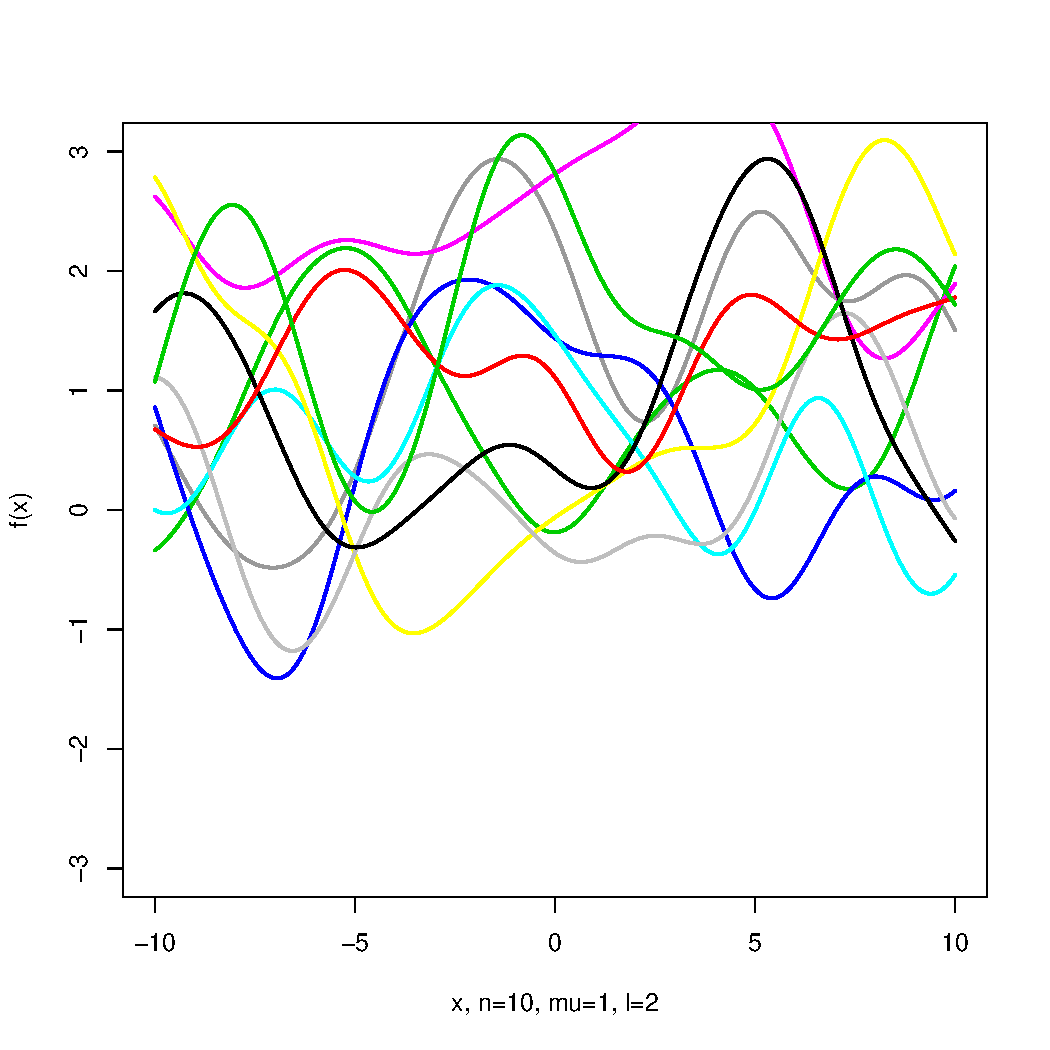
\includegraphics[scale=0.2]{hw321/n10-m1-l2.pdf}
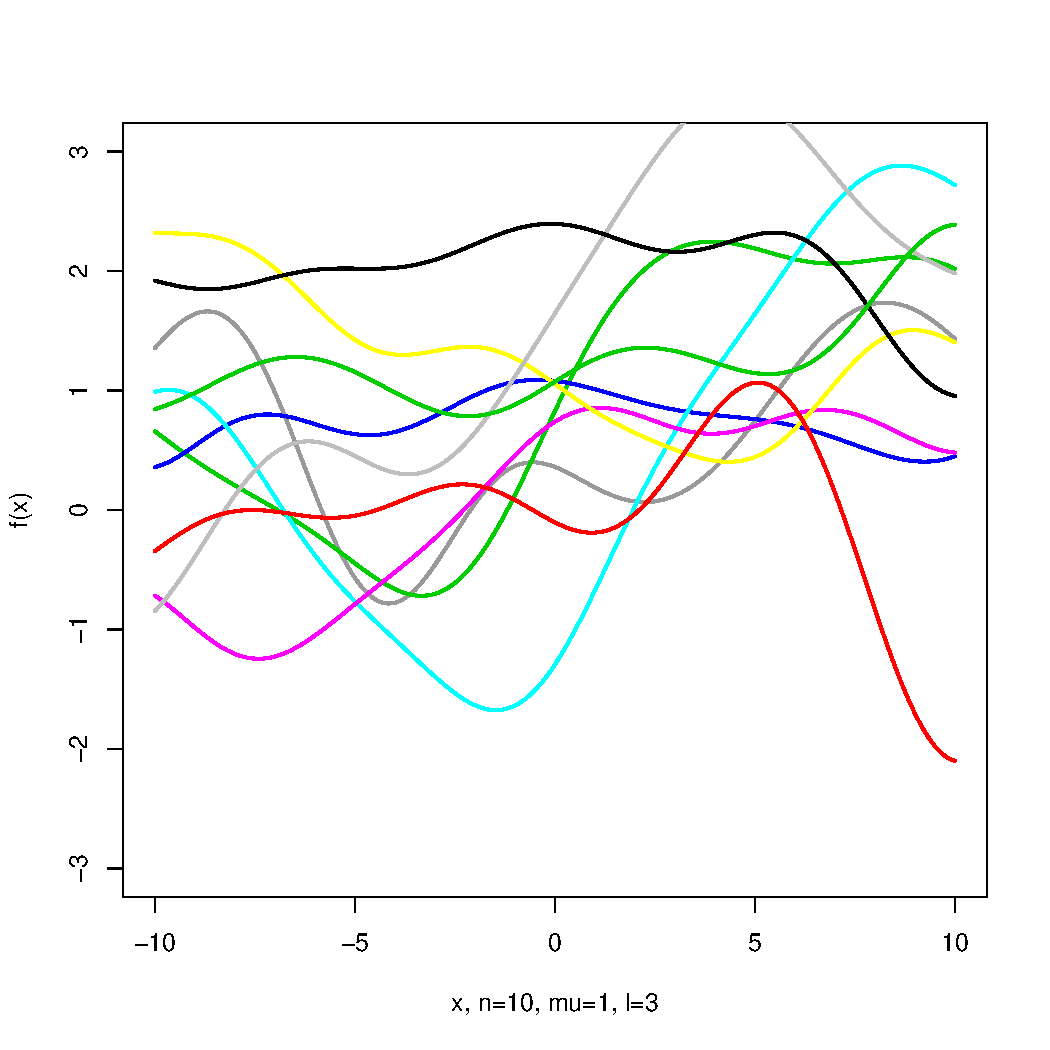
\includegraphics[scale=0.2]{hw321/n10-m1-l3.pdf}
\end{center}
\end{figure}

\pagebreak
\section{Rational Quadratic Covariance}

The simulations in this section use the rational quadratic covariance function:
\begin{eqnarray*}
k(x, x^{\prime}) &=& (1 + \frac{ {(x - x^{\prime})^2} }{ 2 \alpha \ell^2  })^{-\alpha}
\end{eqnarray*} 

The parameters of interest here are the same as above with the addition of $\alpha$. The tuple $(\alpha, \ell)$ can be seen as a scale mixture. 

\begin{figure}
\begin{center}
\includegraphics[scale=0.2]{hw321/n3-m-1-l1-a1.pdf}
\includegraphics[scale=0.2]{hw321/n3-m-1-l1-a4.pdf}
\includegraphics[scale=0.2]{hw321/n3-m-1-l1-a6.pdf}
\includegraphics[scale=0.2]{hw321/n3-m-1-l2-a1.pdf}
\includegraphics[scale=0.2]{hw321/n3-m-1-l2-a4.pdf}
\includegraphics[scale=0.2]{hw321/n3-m-1-l2-a6.pdf}
\includegraphics[scale=0.2]{hw321/n3-m-1-l3-a1.pdf}
\includegraphics[scale=0.2]{hw321/n3-m-1-l3-a4.pdf}
\includegraphics[scale=0.2]{hw321/n3-m-1-l3-a6.pdf}
\end{center}
\end{figure}
\begin{figure}
\begin{center}
\includegraphics[scale=0.2]{hw321/n3-m0-l1-a1.pdf}
\includegraphics[scale=0.2]{hw321/n3-m0-l1-a4.pdf}
\includegraphics[scale=0.2]{hw321/n3-m0-l1-a6.pdf}
\includegraphics[scale=0.2]{hw321/n3-m0-l2-a1.pdf}
\includegraphics[scale=0.2]{hw321/n3-m0-l2-a4.pdf}
\includegraphics[scale=0.2]{hw321/n3-m0-l2-a6.pdf}
\includegraphics[scale=0.2]{hw321/n3-m0-l3-a1.pdf}
\includegraphics[scale=0.2]{hw321/n3-m0-l3-a4.pdf}
\includegraphics[scale=0.2]{hw321/n3-m0-l3-a6.pdf}
\end{center}
\end{figure}
\begin{figure}
\begin{center}
\includegraphics[scale=0.2]{hw321/n3-m1-l1-a1.pdf}
\includegraphics[scale=0.2]{hw321/n3-m1-l1-a4.pdf}
\includegraphics[scale=0.2]{hw321/n3-m1-l1-a6.pdf}
\includegraphics[scale=0.2]{hw321/n3-m1-l2-a1.pdf}
\includegraphics[scale=0.2]{hw321/n3-m1-l2-a4.pdf}
\includegraphics[scale=0.2]{hw321/n3-m1-l2-a6.pdf}
\includegraphics[scale=0.2]{hw321/n3-m1-l3-a1.pdf}
\includegraphics[scale=0.2]{hw321/n3-m1-l3-a4.pdf}
\includegraphics[scale=0.2]{hw321/n3-m1-l3-a6.pdf}
\end{center}
\end{figure}
\begin{figure}
\begin{center}
\includegraphics[scale=0.2]{hw321/n5-m-1-l1-a1.pdf}
\includegraphics[scale=0.2]{hw321/n5-m-1-l1-a4.pdf}
\includegraphics[scale=0.2]{hw321/n5-m-1-l1-a6.pdf}
\includegraphics[scale=0.2]{hw321/n5-m-1-l2-a1.pdf}
\includegraphics[scale=0.2]{hw321/n5-m-1-l2-a4.pdf}
\includegraphics[scale=0.2]{hw321/n5-m-1-l2-a6.pdf}
\includegraphics[scale=0.2]{hw321/n5-m-1-l3-a1.pdf}
\includegraphics[scale=0.2]{hw321/n5-m-1-l3-a4.pdf}
\includegraphics[scale=0.2]{hw321/n5-m-1-l3-a6.pdf}
\end{center}
\end{figure}
\begin{figure}
\begin{center}
\includegraphics[scale=0.2]{hw321/n5-m0-l1-a1.pdf}
\includegraphics[scale=0.2]{hw321/n5-m0-l1-a4.pdf}
\includegraphics[scale=0.2]{hw321/n5-m0-l1-a6.pdf}
\includegraphics[scale=0.2]{hw321/n5-m0-l2-a1.pdf}
\includegraphics[scale=0.2]{hw321/n5-m0-l2-a4.pdf}
\includegraphics[scale=0.2]{hw321/n5-m0-l2-a6.pdf}
\includegraphics[scale=0.2]{hw321/n5-m0-l3-a1.pdf}
\includegraphics[scale=0.2]{hw321/n5-m0-l3-a4.pdf}
\includegraphics[scale=0.2]{hw321/n5-m0-l3-a6.pdf}
\end{center}
\end{figure}
\begin{figure}
\begin{center}
\includegraphics[scale=0.2]{hw321/n5-m1-l1-a1.pdf}
\includegraphics[scale=0.2]{hw321/n5-m1-l1-a4.pdf}
\includegraphics[scale=0.2]{hw321/n5-m1-l1-a6.pdf}
\includegraphics[scale=0.2]{hw321/n5-m1-l2-a1.pdf}
\includegraphics[scale=0.2]{hw321/n5-m1-l2-a4.pdf}
\includegraphics[scale=0.2]{hw321/n5-m1-l2-a6.pdf}
\includegraphics[scale=0.2]{hw321/n5-m1-l3-a1.pdf}
\includegraphics[scale=0.2]{hw321/n5-m1-l3-a4.pdf}
\includegraphics[scale=0.2]{hw321/n5-m1-l3-a6.pdf}
\end{center}
\end{figure}
\begin{figure}
\begin{center}
\includegraphics[scale=0.2]{hw321/n10-m-1-l1-a1.pdf}
\includegraphics[scale=0.2]{hw321/n10-m-1-l1-a4.pdf}
\includegraphics[scale=0.2]{hw321/n10-m-1-l1-a6.pdf}
\includegraphics[scale=0.2]{hw321/n10-m-1-l2-a1.pdf}
\includegraphics[scale=0.2]{hw321/n10-m-1-l2-a4.pdf}
\includegraphics[scale=0.2]{hw321/n10-m-1-l2-a6.pdf}
\includegraphics[scale=0.2]{hw321/n10-m-1-l3-a1.pdf}
\includegraphics[scale=0.2]{hw321/n10-m-1-l3-a4.pdf}
\includegraphics[scale=0.2]{hw321/n10-m-1-l3-a6.pdf}
\end{center}
\end{figure}
\begin{figure}
\begin{center}
\includegraphics[scale=0.2]{hw321/n10-m0-l1-a1.pdf}
\includegraphics[scale=0.2]{hw321/n10-m0-l1-a4.pdf}
\includegraphics[scale=0.2]{hw321/n10-m0-l1-a6.pdf}
\includegraphics[scale=0.2]{hw321/n10-m0-l2-a1.pdf}
\includegraphics[scale=0.2]{hw321/n10-m0-l2-a4.pdf}
\includegraphics[scale=0.2]{hw321/n10-m0-l2-a6.pdf}
\includegraphics[scale=0.2]{hw321/n10-m0-l3-a1.pdf}
\includegraphics[scale=0.2]{hw321/n10-m0-l3-a4.pdf}
\includegraphics[scale=0.2]{hw321/n10-m0-l3-a6.pdf}
\end{center}
\end{figure}
\begin{figure}
\begin{center}
\includegraphics[scale=0.2]{hw321/n10-m1-l1-a1.pdf}
\includegraphics[scale=0.2]{hw321/n10-m1-l1-a4.pdf}
\includegraphics[scale=0.2]{hw321/n10-m1-l1-a6.pdf}
\includegraphics[scale=0.2]{hw321/n10-m1-l2-a1.pdf}
\includegraphics[scale=0.2]{hw321/n10-m1-l2-a4.pdf}
\includegraphics[scale=0.2]{hw321/n10-m1-l2-a6.pdf}
\includegraphics[scale=0.2]{hw321/n10-m1-l3-a1.pdf}
\includegraphics[scale=0.2]{hw321/n10-m1-l3-a4.pdf}
\includegraphics[scale=0.2]{hw321/n10-m1-l3-a6.pdf}
\end{center}
\end{figure}


\pagebreak
\section{$\gamma$-Exponential Covariance}

The simulations in this section use the $\gamma$-exponential covariance function:
\begin{eqnarray*}
% k(x, x^{\prime}) &=& (1 + \frac{ {(x - x^{\prime})^2 } }{ 2 \alpha \ell^2  })^{-\alpha}
k(x, x^{\prime}) &=& \exp \{ - (\frac{x - x^{\prime}}{\ell})^{\gamma} \}
\end{eqnarray*} 

The parameters of interest here are the same as the squared exponential, with the addition of $\gamma$. This is a more general class of covariance function, of which the exponential and squared exponential are special cases.

\begin{figure}
\begin{center}
\includegraphics[scale=0.2]{hw321/n3-m-1-l1-g1.pdf}
\includegraphics[scale=0.2]{hw321/n3-m-1-l1-g2.pdf}
\includegraphics[scale=0.2]{hw321/n3-m-1-l1-g4.pdf}
\includegraphics[scale=0.2]{hw321/n3-m-1-l2-g1.pdf}
\includegraphics[scale=0.2]{hw321/n3-m-1-l2-g2.pdf}
\includegraphics[scale=0.2]{hw321/n3-m-1-l2-g4.pdf}
\includegraphics[scale=0.2]{hw321/n3-m-1-l3-g1.pdf}
\includegraphics[scale=0.2]{hw321/n3-m-1-l3-g2.pdf}
\includegraphics[scale=0.2]{hw321/n3-m-1-l3-g4.pdf}
\end{center}
\end{figure}
\begin{figure}
\begin{center}
\includegraphics[scale=0.2]{hw321/n3-m0-l1-g1.pdf}
\includegraphics[scale=0.2]{hw321/n3-m0-l1-g2.pdf}
\includegraphics[scale=0.2]{hw321/n3-m0-l1-g4.pdf}
\includegraphics[scale=0.2]{hw321/n3-m0-l2-g1.pdf}
\includegraphics[scale=0.2]{hw321/n3-m0-l2-g2.pdf}
\includegraphics[scale=0.2]{hw321/n3-m0-l2-g4.pdf}
\includegraphics[scale=0.2]{hw321/n3-m0-l3-g1.pdf}
\includegraphics[scale=0.2]{hw321/n3-m0-l3-g2.pdf}
\includegraphics[scale=0.2]{hw321/n3-m0-l3-g4.pdf}
\end{center}
\end{figure}
\begin{figure}
\begin{center}
\includegraphics[scale=0.2]{hw321/n3-m1-l1-g1.pdf}
\includegraphics[scale=0.2]{hw321/n3-m1-l1-g2.pdf}
\includegraphics[scale=0.2]{hw321/n3-m1-l1-g4.pdf}
\includegraphics[scale=0.2]{hw321/n3-m1-l2-g1.pdf}
\includegraphics[scale=0.2]{hw321/n3-m1-l2-g2.pdf}
\includegraphics[scale=0.2]{hw321/n3-m1-l2-g4.pdf}
\includegraphics[scale=0.2]{hw321/n3-m1-l3-g1.pdf}
\includegraphics[scale=0.2]{hw321/n3-m1-l3-g2.pdf}
\includegraphics[scale=0.2]{hw321/n3-m1-l3-g4.pdf}
\end{center}
\end{figure}
\begin{figure}
\begin{center}
\includegraphics[scale=0.2]{hw321/n5-m-1-l1-g1.pdf}
\includegraphics[scale=0.2]{hw321/n5-m-1-l1-g2.pdf}
\includegraphics[scale=0.2]{hw321/n5-m-1-l1-g4.pdf}
\includegraphics[scale=0.2]{hw321/n5-m-1-l2-g1.pdf}
\includegraphics[scale=0.2]{hw321/n5-m-1-l2-g2.pdf}
\includegraphics[scale=0.2]{hw321/n5-m-1-l2-g4.pdf}
\includegraphics[scale=0.2]{hw321/n5-m-1-l3-g1.pdf}
\includegraphics[scale=0.2]{hw321/n5-m-1-l3-g2.pdf}
\includegraphics[scale=0.2]{hw321/n5-m-1-l3-g4.pdf}
\end{center}
\end{figure}
\begin{figure}
\begin{center}
\includegraphics[scale=0.2]{hw321/n5-m0-l1-g1.pdf}
\includegraphics[scale=0.2]{hw321/n5-m0-l1-g2.pdf}
\includegraphics[scale=0.2]{hw321/n5-m0-l1-g4.pdf}
\includegraphics[scale=0.2]{hw321/n5-m0-l2-g1.pdf}
\includegraphics[scale=0.2]{hw321/n5-m0-l2-g2.pdf}
\includegraphics[scale=0.2]{hw321/n5-m0-l2-g4.pdf}
\includegraphics[scale=0.2]{hw321/n5-m0-l3-g1.pdf}
\includegraphics[scale=0.2]{hw321/n5-m0-l3-g2.pdf}
\includegraphics[scale=0.2]{hw321/n5-m0-l3-g4.pdf}
\end{center}
\end{figure}
\begin{figure}
\begin{center}
\includegraphics[scale=0.2]{hw321/n5-m1-l1-g1.pdf}
\includegraphics[scale=0.2]{hw321/n5-m1-l1-g2.pdf}
\includegraphics[scale=0.2]{hw321/n5-m1-l1-g4.pdf}
\includegraphics[scale=0.2]{hw321/n5-m1-l2-g1.pdf}
\includegraphics[scale=0.2]{hw321/n5-m1-l2-g2.pdf}
\includegraphics[scale=0.2]{hw321/n5-m1-l2-g4.pdf}
\includegraphics[scale=0.2]{hw321/n5-m1-l3-g1.pdf}
\includegraphics[scale=0.2]{hw321/n5-m1-l3-g2.pdf}
\includegraphics[scale=0.2]{hw321/n5-m1-l3-g4.pdf}
\end{center}
\end{figure}
\begin{figure}
\begin{center}
\includegraphics[scale=0.2]{hw321/n10-m-1-l1-g1.pdf}
\includegraphics[scale=0.2]{hw321/n10-m-1-l1-g2.pdf}
\includegraphics[scale=0.2]{hw321/n10-m-1-l1-g4.pdf}
\includegraphics[scale=0.2]{hw321/n10-m-1-l2-g1.pdf}
\includegraphics[scale=0.2]{hw321/n10-m-1-l2-g2.pdf}
\includegraphics[scale=0.2]{hw321/n10-m-1-l2-g4.pdf}
\includegraphics[scale=0.2]{hw321/n10-m-1-l3-g1.pdf}
\includegraphics[scale=0.2]{hw321/n10-m-1-l3-g2.pdf}
\includegraphics[scale=0.2]{hw321/n10-m-1-l3-g4.pdf}
\end{center}
\end{figure}
\begin{figure}
\begin{center}
\includegraphics[scale=0.2]{hw321/n10-m0-l1-g1.pdf}
\includegraphics[scale=0.2]{hw321/n10-m0-l1-g2.pdf}
\includegraphics[scale=0.2]{hw321/n10-m0-l1-g4.pdf}
\includegraphics[scale=0.2]{hw321/n10-m0-l2-g1.pdf}
\includegraphics[scale=0.2]{hw321/n10-m0-l2-g2.pdf}
\includegraphics[scale=0.2]{hw321/n10-m0-l2-g4.pdf}
\includegraphics[scale=0.2]{hw321/n10-m0-l3-g1.pdf}
\includegraphics[scale=0.2]{hw321/n10-m0-l3-g2.pdf}
\includegraphics[scale=0.2]{hw321/n10-m0-l3-g4.pdf}
\end{center}
\end{figure}
\begin{figure}
\begin{center}
\includegraphics[scale=0.2]{hw321/n10-m1-l1-g1.pdf}
\includegraphics[scale=0.2]{hw321/n10-m1-l1-g2.pdf}
\includegraphics[scale=0.2]{hw321/n10-m1-l1-g4.pdf}
\includegraphics[scale=0.2]{hw321/n10-m1-l2-g1.pdf}
\includegraphics[scale=0.2]{hw321/n10-m1-l2-g2.pdf}
\includegraphics[scale=0.2]{hw321/n10-m1-l2-g4.pdf}
\includegraphics[scale=0.2]{hw321/n10-m1-l3-g1.pdf}
\includegraphics[scale=0.2]{hw321/n10-m1-l3-g2.pdf}
\includegraphics[scale=0.2]{hw321/n10-m1-l3-g4.pdf}
\end{center}
\end{figure} 

\end{document}
